\documentclass[sigconf, natbib=false, nonacm]{acmart}  
%DIF LATEXDIFF DIFFERENCE FILE


\setcopyright{none}
\settopmatter{printacmref=false}
\def\@copyrightspace{\relax}
\settopmatter{printacmref=false} % Removes citation information below abstract
\renewcommand\footnotetextcopyrightpermission[1]{} % removes footnote with conference information in first column

% see also ### ACM template on overleaf 
\usepackage[
backend=biber,
style=numeric,
sorting=ynt,
]{biblatex}
\bibliography{references.bib}


\usepackage{pdfpages} % http://mirror.unl.edu/ctan/macros/latex/contrib/pdfpages/pdfpages.pdf
\usepackage{booktabs}
\usepackage{balance}
\usepackage{enumitem}
\usepackage{lscape}

%DIF 23a23-24
\usepackage{listings} %DIF > 
 %DIF > 
%DIF -------
\usepackage{lineno}
% \linenumbers  

\usepackage[utf8]{inputenc}
\usepackage{amsmath}
\usepackage{graphicx}

\pagestyle{plain} % removes running headers

\usepackage[colorinlistoftodos]{todonotes} % handig voor commentaar: gebruik \todo{}, zie ftp://ftp.fu-berlin.de/tex/CTAN/macros/latex/contrib/todonotes/todonotes.pdf
\usepackage{listings}
\usepackage{pdfpages}
%DIF 35a37
\usepackage{adjustbox} %DIF > 
%DIF -------
\usepackage{tcolorbox}
\usepackage{float}
%DIF 37a40
\usepackage{tikzpagenodes} %DIF > 
%DIF -------
\usepackage{caption}
\usepackage{wrapfig}
\usepackage{subcaption}

\usepackage{hyperref}


% when writing in Dutch
%\usepackage[dutch]{babel}
%\selectlanguage{dutch}
%DIF PREAMBLE EXTENSION ADDED BY LATEXDIFF
%DIF UNDERLINE PREAMBLE %DIF PREAMBLE
\RequirePackage[normalem]{ulem} %DIF PREAMBLE
\RequirePackage{color}\definecolor{RED}{rgb}{1,0,0}\definecolor{BLUE}{rgb}{0,0,1} %DIF PREAMBLE
\providecommand{\DIFaddtex}[1]{{\protect\color{blue}\uwave{#1}}} %DIF PREAMBLE
\providecommand{\DIFdeltex}[1]{{\protect\color{red}\sout{#1}}}                      %DIF PREAMBLE
%DIF SAFE PREAMBLE %DIF PREAMBLE
\providecommand{\DIFaddbegin}{} %DIF PREAMBLE
\providecommand{\DIFaddend}{} %DIF PREAMBLE
\providecommand{\DIFdelbegin}{} %DIF PREAMBLE
\providecommand{\DIFdelend}{} %DIF PREAMBLE
%DIF FLOATSAFE PREAMBLE %DIF PREAMBLE
\providecommand{\DIFaddFL}[1]{\DIFadd{#1}} %DIF PREAMBLE
\providecommand{\DIFdelFL}[1]{\DIFdel{#1}} %DIF PREAMBLE
\providecommand{\DIFaddbeginFL}{} %DIF PREAMBLE
\providecommand{\DIFaddendFL}{} %DIF PREAMBLE
\providecommand{\DIFdelbeginFL}{} %DIF PREAMBLE
\providecommand{\DIFdelendFL}{} %DIF PREAMBLE
%DIF HYPERREF PREAMBLE %DIF PREAMBLE
\providecommand{\DIFadd}[1]{\texorpdfstring{\DIFaddtex{#1}}{#1}} %DIF PREAMBLE
\providecommand{\DIFdel}[1]{\texorpdfstring{\DIFdeltex{#1}}{}} %DIF PREAMBLE
\newcommand{\DIFscaledelfig}{0.5}
%DIF HIGHLIGHTGRAPHICS PREAMBLE %DIF PREAMBLE
\RequirePackage{settobox} %DIF PREAMBLE
\RequirePackage{letltxmacro} %DIF PREAMBLE
\newsavebox{\DIFdelgraphicsbox} %DIF PREAMBLE
\newlength{\DIFdelgraphicswidth} %DIF PREAMBLE
\newlength{\DIFdelgraphicsheight} %DIF PREAMBLE
% store original definition of \includegraphics %DIF PREAMBLE
\LetLtxMacro{\DIFOincludegraphics}{\includegraphics} %DIF PREAMBLE
\newcommand{\DIFaddincludegraphics}[2][]{{\color{blue}\fbox{\DIFOincludegraphics[#1]{#2}}}} %DIF PREAMBLE
\newcommand{\DIFdelincludegraphics}[2][]{% %DIF PREAMBLE
\sbox{\DIFdelgraphicsbox}{\DIFOincludegraphics[#1]{#2}}% %DIF PREAMBLE
\settoboxwidth{\DIFdelgraphicswidth}{\DIFdelgraphicsbox} %DIF PREAMBLE
\settoboxtotalheight{\DIFdelgraphicsheight}{\DIFdelgraphicsbox} %DIF PREAMBLE
\scalebox{\DIFscaledelfig}{% %DIF PREAMBLE
\parbox[b]{\DIFdelgraphicswidth}{\usebox{\DIFdelgraphicsbox}\\[-\baselineskip] \rule{\DIFdelgraphicswidth}{0em}}\llap{\resizebox{\DIFdelgraphicswidth}{\DIFdelgraphicsheight}{% %DIF PREAMBLE
\setlength{\unitlength}{\DIFdelgraphicswidth}% %DIF PREAMBLE
\begin{picture}(1,1)% %DIF PREAMBLE
\thicklines\linethickness{2pt} %DIF PREAMBLE
{\color[rgb]{1,0,0}\put(0,0){\framebox(1,1){}}}% %DIF PREAMBLE
{\color[rgb]{1,0,0}\put(0,0){\line( 1,1){1}}}% %DIF PREAMBLE
{\color[rgb]{1,0,0}\put(0,1){\line(1,-1){1}}}% %DIF PREAMBLE
\end{picture}% %DIF PREAMBLE
}\hspace*{3pt}}} %DIF PREAMBLE
} %DIF PREAMBLE
\LetLtxMacro{\DIFOaddbegin}{\DIFaddbegin} %DIF PREAMBLE
\LetLtxMacro{\DIFOaddend}{\DIFaddend} %DIF PREAMBLE
\LetLtxMacro{\DIFOdelbegin}{\DIFdelbegin} %DIF PREAMBLE
\LetLtxMacro{\DIFOdelend}{\DIFdelend} %DIF PREAMBLE
\DeclareRobustCommand{\DIFaddbegin}{\DIFOaddbegin \let\includegraphics\DIFaddincludegraphics} %DIF PREAMBLE
\DeclareRobustCommand{\DIFaddend}{\DIFOaddend \let\includegraphics\DIFOincludegraphics} %DIF PREAMBLE
\DeclareRobustCommand{\DIFdelbegin}{\DIFOdelbegin \let\includegraphics\DIFdelincludegraphics} %DIF PREAMBLE
\DeclareRobustCommand{\DIFdelend}{\DIFOaddend \let\includegraphics\DIFOincludegraphics} %DIF PREAMBLE
\LetLtxMacro{\DIFOaddbeginFL}{\DIFaddbeginFL} %DIF PREAMBLE
\LetLtxMacro{\DIFOaddendFL}{\DIFaddendFL} %DIF PREAMBLE
\LetLtxMacro{\DIFOdelbeginFL}{\DIFdelbeginFL} %DIF PREAMBLE
\LetLtxMacro{\DIFOdelendFL}{\DIFdelendFL} %DIF PREAMBLE
\DeclareRobustCommand{\DIFaddbeginFL}{\DIFOaddbeginFL \let\includegraphics\DIFaddincludegraphics} %DIF PREAMBLE
\DeclareRobustCommand{\DIFaddendFL}{\DIFOaddendFL \let\includegraphics\DIFOincludegraphics} %DIF PREAMBLE
\DeclareRobustCommand{\DIFdelbeginFL}{\DIFOdelbeginFL \let\includegraphics\DIFdelincludegraphics} %DIF PREAMBLE
\DeclareRobustCommand{\DIFdelendFL}{\DIFOaddendFL \let\includegraphics\DIFOincludegraphics} %DIF PREAMBLE
%DIF LISTINGS PREAMBLE %DIF PREAMBLE
\RequirePackage{listings} %DIF PREAMBLE
\RequirePackage{color} %DIF PREAMBLE
\lstdefinelanguage{DIFcode}{ %DIF PREAMBLE
%DIF DIFCODE_UNDERLINE %DIF PREAMBLE
  moredelim=[il][\color{red}\sout]{\%DIF\ <\ }, %DIF PREAMBLE
  moredelim=[il][\color{blue}\uwave]{\%DIF\ >\ } %DIF PREAMBLE
} %DIF PREAMBLE
\lstdefinestyle{DIFverbatimstyle}{ %DIF PREAMBLE
	language=DIFcode, %DIF PREAMBLE
	basicstyle=\ttfamily, %DIF PREAMBLE
	columns=fullflexible, %DIF PREAMBLE
	keepspaces=true %DIF PREAMBLE
} %DIF PREAMBLE
\lstnewenvironment{DIFverbatim}{\lstset{style=DIFverbatimstyle}}{} %DIF PREAMBLE
\lstnewenvironment{DIFverbatim*}{\lstset{style=DIFverbatimstyle,showspaces=true}}{} %DIF PREAMBLE
%DIF END PREAMBLE EXTENSION ADDED BY LATEXDIFF

\begin{document}
\pagenumbering{arabic}

\title{Inspecting \DIFaddbegin \DIFadd{Aggregated }\DIFaddend Cycling Attention\DIFaddbegin \DIFadd{: }\\ \DIFadd{Merging multiple eye-trackers}\DIFaddend }
\author{Ivo Cornelis de Geus}
\DIFdelbegin %DIFDELCMD < \keywords{Infrastructure, Smart Mobility, Computer Vision, Eye Tracking, Heatmaps}
%DIFDELCMD < %%%
\DIFdelend \DIFaddbegin \keywords{Infrastructure, Smart Mobility, Computer Vision, Eye-Tracking, Heatmaps}
\DIFaddend 

\begin{abstract}
    As cycling is increasingly adopted as the future of sustainable \DIFdelbegin \DIFdel{human }\DIFdelend mobility, governments are \DIFdelbegin \DIFdel{increasingly }\DIFdelend interested in making it safer. \DIFdelbegin \DIFdel{During }\DIFdelend \DIFaddbegin \DIFadd{We use various senses during }\DIFaddend any traffic interaction, \DIFdelbegin \DIFdel{we use a variety of senses to direct us, of }\DIFdelend \DIFaddbegin \DIFadd{of }\DIFaddend which the visual is the most dominant. \DIFdelbegin \DIFdel{Eye-movement in automotors }\DIFdelend \DIFaddbegin \DIFadd{While eye-movement research in auto-motors }\DIFaddend is a mature field, \DIFdelbegin \DIFdel{while }\DIFdelend the amount of research in cycling is relatively small. This \DIFdelbegin \DIFdel{project aimed to map }\DIFdelend \DIFaddbegin \DIFadd{research maps }\DIFaddend a single wearable \DIFdelbegin \DIFdel{eye trackers to a master video-track using computer vision. With test-footage, several methods of this mapping images together have been tested, of which a Siamese Network performed best, but still with }\DIFdelend \DIFaddbegin \DIFadd{eye-tracker to master footage using computer recognition and evaluates both Scale Invariant Feature Transform (SIFT) and implementation of a Siamese Neural Network (SNN). Of both, SIFT obtained }\DIFaddend an accuracy of \DIFdelbegin \DIFdel{only }\DIFdelend \DIFaddbegin \DIFadd{52\% and the SNN an accuracy of }\DIFaddend 38.6\%. \DIFaddbegin \DIFadd{Both are not robust enough to build a reliable mapping but establish a baseline for future research. 
}\DIFaddend \end{abstract}

\maketitle


%DIF >  \begin{tikzpicture}[remember picture,overlay,shift={(current page.north west)}]
%DIF >  \node[anchor=north west,yshift=0.5cm,xshift=-0.2cm]{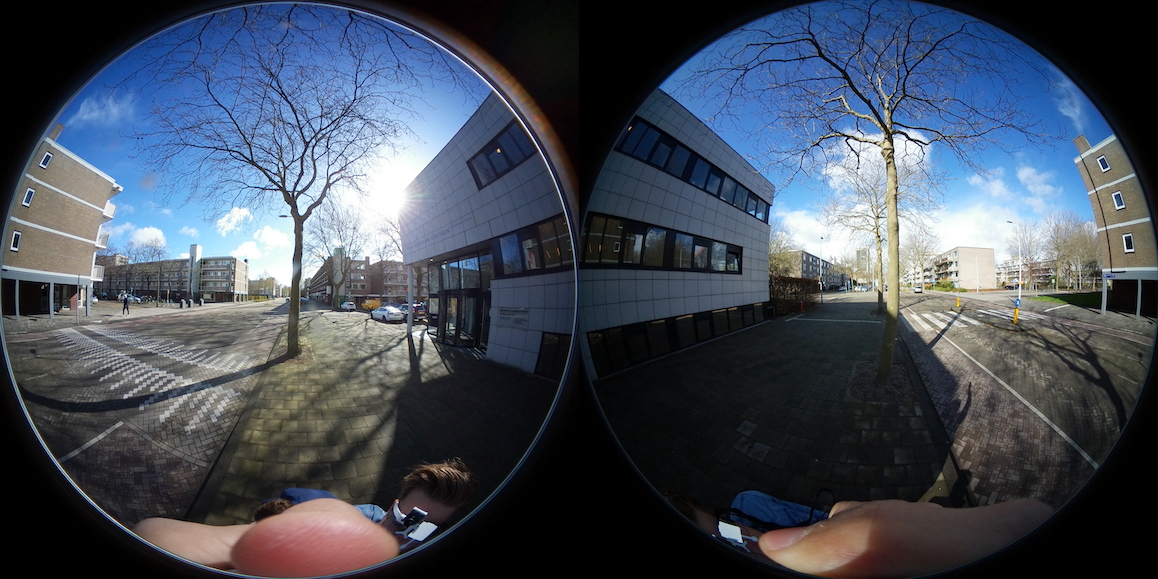
\includegraphics[width=\paperwidth, height=2.2cm]{figures/1 original.JPG}};
%DIF >  \end{tikzpicture}
\DIFaddbegin 


\DIFaddend \begin{description}
     \item[Student] \href{mailto:ivo.de.geus@student.uva.nl}{Ivo Cornelis de Geus}
     \item[External Supervisor] \href{mailto:jschreuder@kexxu.com}{J. Schreuder, PhD}
     \item[External Supervisor] \href{mailto:sander.buningh@bam.com}{S. Buningh, Ir. }
     \item[Internal Supervisor] \href{mailto:m.worring@uva.nl}{Prof. Dr. M. Worring}
     \DIFdelbegin %DIFDELCMD < \item[Github] \url{https://github.com/idegeus/msc-ds-thesis}
\item[\DIFdel{Github}]%DIFAUXCMD
%DIFDELCMD < %%%
\DIFdelend \DIFaddbegin \item[Thesis Repo] \href{https://github.com/idegeus/msc-ds-thesis}{idegeus/msc-ds-thesis}
     \item[Python Repo] \href{https://github.com/kexxu-robotics/video_heatmap}{kexxu-robotics/video\_heatmap}
     \item[Video Footage] \href{https://youtube.com/playlist?list=PLzh4mA3kUCz2J9pJhzKEI88LiCYvB9BQk}{Playlist Link}
\DIFaddend \end{description} 

\section{Introduction}
    \DIFdelbegin \DIFdel{Biking }\DIFdelend \DIFaddbegin \subsection{\DIFadd{Cycling \& Traffic Attention}}
    \DIFadd{Cycling }\DIFaddend is often touted as the future of \DIFdelbegin \DIFdel{individual mobilityto replace cars}\DIFdelend \DIFaddbegin \DIFadd{personal mobility}\DIFaddend , with good reason\DIFdelbegin \DIFdel{. It's }\DIFdelend \DIFaddbegin \DIFadd{: it is }\DIFaddend healthy, cheap, fun, and good for the environment \cite{DeGeus2009, Hendriksen2010, St-Louis2014}. From \DIFdelbegin \DIFdel{the perspective of a government}\DIFdelend \DIFaddbegin \DIFadd{a governments' perspective}\DIFaddend , citizens get significantly healthier, \DIFaddbegin \DIFadd{which is }\DIFaddend combined with a more efficient spatial urban \DIFdelbegin \DIFdel{design \mbox{%DIFAUXCMD
\cite{}}\hspace{0pt}%DIFAUXCMD
}\DIFdelend \DIFaddbegin \DIFadd{character \mbox{%DIFAUXCMD
\cite{Nello-Deakin2019, Bruun1995}}\hspace{0pt}%DIFAUXCMD
}\DIFaddend . With 68\% of the world population expected to live in urban areas by 2050, \DIFdelbegin \DIFdel{biking is deemed such a promising }\DIFdelend \DIFaddbegin \DIFadd{the United Nations deems Cycling such a good }\DIFaddend fit in its sustainability goals that \DIFdelbegin \DIFdel{the United Nations }\DIFdelend \DIFaddbegin \DIFadd{it }\DIFaddend declared the third of June as the \DIFdelbegin \DIFdel{day of the bike }\DIFdelend \DIFaddbegin \DIFadd{international cycling day }\DIFaddend \cite{UnitedNations2019, UnitedNations2018a, UnitedNations2018}.
    \DIFdelbegin \DIFdel{\#BanCars
    }\DIFdelend 

    \DIFdelbegin \DIFdel{To get everyone on the bike and create a welcoming built environment for biking}\DIFdelend \DIFaddbegin \DIFadd{In aiming for these advantages}\DIFaddend , governments are increasingly looking for advice to countries with \DIFdelbegin \DIFdel{an existing prominent biking culture, such as }\DIFdelend \DIFaddbegin \DIFadd{success stories in creating a cycling culture. Examples of these countries are }\DIFaddend the Netherlands, Denmark, and Germany \cite{Schepers2017}. An increasingly discussed \DIFdelbegin \DIFdel{, but equally controversial, }\DIFdelend measure to improve the "\DIFdelbegin \DIFdel{biking }\DIFdelend \DIFaddbegin \DIFadd{cycling }\DIFaddend climate" is a redistribution of urban space to prioritize one modality over the other \cite{Nello-Deakin2019, Gossling2020}. 

    Equally \DIFdelbegin \DIFdel{important }\DIFdelend \DIFaddbegin \DIFadd{crucial }\DIFaddend as linked to the urban decisions is \DIFdelbegin \DIFdel{the environment in which }\DIFdelend \DIFaddbegin \DIFadd{how }\DIFaddend transport is taking place and how it is perceived. \DIFdelbegin \DIFdel{Since the visual perception is the most important factor in navigation and perceptual errors contribute 20\% of European road accidents, it makes sense to see how we process this information \mbox{%DIFAUXCMD
\cite{ERSO2020}}\hspace{0pt}%DIFAUXCMD
. \mbox{%DIFAUXCMD
\citeauthor{ERSO2020} }\hspace{0pt}%DIFAUXCMD
claims that in 2020, biking is the only modality not decreasing in fatalities since 2010, therefore it makes sense to pay attention to where bikers are looking and how they are paying attention. }%DIFDELCMD < 

%DIFDELCMD <     %%%
\DIFdelend \DIFaddbegin \DIFadd{When people navigate public spaces, they scan their surroundings mostly unconsciously to adapt and fit in in traffic \mbox{%DIFAUXCMD
\cite{HollanderJustinB.Sussman}}\hspace{0pt}%DIFAUXCMD
. }\DIFaddend In a historical perspective\DIFdelbegin \DIFdel{of using eye movements}\DIFdelend , \citeauthor{VanGompel2007} refer to Du Laurens, a French anatomist and medical scientist in 1596\DIFdelbegin \DIFdel{, who }\DIFdelend \DIFaddbegin \DIFadd{: Du Laurens }\DIFaddend described the eyes as \DIFdelbegin \emph{\DIFdel{windowes of the mind}}%DIFAUXCMD
\DIFdelend \DIFaddbegin \DIFadd{"windows of the mind"}\DIFaddend . Indeed, it seems clear today that eye movements reveal the workings of the mind and the brain \cite{VanGompel2007}. \DIFdelbegin \DIFdel{The theory that eyes give }\DIFdelend \DIFaddbegin \DIFadd{\mbox{%DIFAUXCMD
\citeauthor{Just1980} }\hspace{0pt}%DIFAUXCMD
names the the theory on eyes giving }\DIFaddend information about what the brain is \DIFdelbegin \DIFdel{working on is sometimes referred to as the }\DIFdelend \DIFaddbegin \DIFadd{processing the "}\DIFaddend eye-mind assumption\DIFdelbegin \DIFdel{, and while it }\DIFdelend \DIFaddbegin \DIFadd{" \mbox{%DIFAUXCMD
\cite{Just1980}}\hspace{0pt}%DIFAUXCMD
. While this link }\DIFaddend does not directly guarantee processing by the brain, it is still \DIFdelbegin \DIFdel{a robust and useful link \mbox{%DIFAUXCMD
\cite{Just1980, Berger2018}}\hspace{0pt}%DIFAUXCMD
. 
    Because of this, eye-tracking has been widely deployed in multiple fields, ranging from tourism and user testing to software engineering and traffic evaluation \mbox{%DIFAUXCMD
\cite{Liu2011}}\hspace{0pt}%DIFAUXCMD
. While eye-tracking had always been used in a fixed environment, such as a desktop, innovations in wearable electronics allow for researching eye-tracking in a more natural setting. With this comes the trouble of inspecting different participants in a single go, which is what this project will focus on.
    }\DIFdelend \DIFaddbegin \DIFadd{strong and valuable indicator \mbox{%DIFAUXCMD
\cite{Berger2018}}\hspace{0pt}%DIFAUXCMD
. 
    }\DIFaddend 

    \DIFdelbegin \DIFdel{In this research, an attempt is made to set up a method to map a wearable eye tracker on one single master image using a computer vision feature detection system. Normal eye trackers in a controlled environment are mapped onto one single master image in 360 degrees called a map of Areas of Interest (AOI). In this way, it could become clear what a group of participants are collectively looking at. This is not possible in a more natural setting where eye trackers are worn in a wearable form. 
  }%DIFDELCMD < 

%DIFDELCMD < %%%
\section{\DIFdel{Background}}
    %DIFAUXCMD
\addtocounter{section}{-1}%DIFAUXCMD
%DIFDELCMD < 

%DIFDELCMD <     %%%
\subsection{\DIFdel{eye tracker}}
        %DIFAUXCMD
\addtocounter{subsection}{-1}%DIFAUXCMD
\DIFdel{In navigating everyday traffic, using human visual information processing is our primary way of getting around safely \mbox{%DIFAUXCMD
\cite{Reyes2008, VanGompel2007, Underwood2007}}\hspace{0pt}%DIFAUXCMD
}\DIFdelend \DIFaddbegin \DIFadd{Since this visual perception is the most crucial factor in navigation and perceptual errors make up 20\% of European road accidents, it makes sense to see how we process this information \mbox{%DIFAUXCMD
\cite{ERSO2020, Reyes2008, VanGompel2007, Underwood2007}}\hspace{0pt}%DIFAUXCMD
}\DIFaddend . It is an \DIFdelbegin \DIFdel{important }\DIFdelend \DIFaddbegin \DIFadd{essential }\DIFaddend factor in obstacle avoidance, safe navigation, and risk perception \DIFdelbegin \DIFdel{, }\DIFdelend and is, therefore, a large part of the required workload \cite{Lehtonen2014, Werneke2012}. \DIFdelbegin \DIFdel{For this reason, }\DIFdelend \DIFaddbegin \DIFadd{Using }\DIFaddend eye-tracking \DIFdelbegin \DIFdel{has been used }\DIFdelend in traffic studies \DIFdelbegin \DIFdel{for a long time. Both }\DIFdelend \DIFaddbegin \DIFadd{is therefore not a new idea: both }\DIFaddend for in car-driving and walking, eye movements \DIFdelbegin \DIFdel{have been }\DIFdelend \DIFaddbegin \DIFadd{are }\DIFaddend studied extensively to evaluate driver awareness \cite{Stapel2020}, intersection design \cite{Werneke2012, Crundall2011}, location, colors\DIFdelbegin \DIFdel{and font }\DIFdelend \DIFaddbegin \DIFadd{, fonts }\DIFaddend of signage \cite{HollanderJustinB.Sussman}, and the impact of information in advanced driver assistant systems \cite{Reyes2008, Kohl2020, OsbeckEmelieAkerman2010}\DIFdelbegin \DIFdel{. Some studies have also tried using }\DIFdelend \DIFaddbegin \DIFadd{, to name but a few.  While \mbox{%DIFAUXCMD
\cite{OsbeckEmelieAkerman2010} }\hspace{0pt}%DIFAUXCMD
argues }\DIFaddend eye-tracking \DIFdelbegin \DIFdel{as a measure of workload and comfort \mbox{%DIFAUXCMD
\cite{Berger2018}}\hspace{0pt}%DIFAUXCMD
.  While some studies argue eye-tracking }\DIFdelend is not sensitive enough to be used for workload measuring\DIFdelbegin \DIFdel{\mbox{%DIFAUXCMD
\cite{OsbeckEmelieAkerman2010}}\hspace{0pt}%DIFAUXCMD
}\DIFdelend , it has sometimes been used to determine behavior\DIFaddbegin \DIFadd{, comfort, }\DIFaddend and workload in traffic situations \DIFdelbegin \DIFdel{\mbox{%DIFAUXCMD
\cite{Mantuano2017a, Cegovnik2018c, Bongiorno2017a}}\hspace{0pt}%DIFAUXCMD
}\DIFdelend \DIFaddbegin \DIFadd{\mbox{%DIFAUXCMD
\cite{Mantuano2017a, Berger2018, Cegovnik2018c, Bongiorno2017a}}\hspace{0pt}%DIFAUXCMD
}\DIFaddend . The amount of research in the visual behavior in \DIFdelbegin \DIFdel{bikers }\DIFdelend \DIFaddbegin \DIFadd{cycling }\DIFaddend (as an urban transport) \DIFdelbegin \DIFdel{was somewhat limited , but }\DIFdelend \DIFaddbegin \DIFadd{used to be limited and }\DIFaddend has seen an \DIFdelbegin \DIFdel{increase }\DIFdelend \DIFaddbegin \DIFadd{uptake }\DIFaddend in recent years \DIFdelbegin \DIFdel{\mbox{%DIFAUXCMD
\cite{Lehtonen2016, Vries2017, Mantuano2017a, Trefzger2018, Kovacsova2018, Rupi2019}}\hspace{0pt}%DIFAUXCMD
. }\DIFdelend \DIFaddbegin \DIFadd{\mbox{%DIFAUXCMD
\cite{Lehtonen2016, Vries2017, Mantuano2017a, Trefzger2018, Kovacsova2018, Rupi2019, HollanderJustinB.Sussman}}\hspace{0pt}%DIFAUXCMD
. This field still holds much potential for further research, as \mbox{%DIFAUXCMD
\citeauthor{ERSO2020} }\hspace{0pt}%DIFAUXCMD
claims that in the period 2010 to 2020, cycling was the only modality not decreasing in fatalities. Cycling is strongly dependent on visual perception in more ways than one, as several studies have shown that even a perceived lack of safety can be a deterrent to cycling \mbox{%DIFAUXCMD
\cite{Fishman2012}}\hspace{0pt}%DIFAUXCMD
. For this reason, it makes sense to pay close attention to where cyclists are looking and how they are paying attention. 
    }\DIFaddend 

    \DIFaddbegin \subsection{\DIFadd{Wearable Eye-Trackers}} %DIF > .
    \DIFaddend Running an eye-tracking experiment on the topic of traffic is possible in a variety of different ways. \DIFdelbegin \DIFdel{In the beginning, running }\DIFdelend \DIFaddbegin \DIFadd{Running }\DIFaddend such an experiment \DIFdelbegin \DIFdel{was mostly }\DIFdelend \DIFaddbegin \DIFadd{is usually }\DIFaddend done in a controlled environment at a desk with a fixed \DIFdelbegin \DIFdel{eye tracker }\DIFdelend \DIFaddbegin \DIFadd{eye-tracker }\DIFaddend such as in \cite{Velichkovsky2003, Werneke2012, Reyes2008}. While this has many advantages\DIFaddbegin \DIFadd{, }\DIFaddend such as internal validity, reliability, and ethical advances, a possible lack of realism and ecological validity of a desk-mounted \DIFdelbegin \DIFdel{eye tracker }\DIFdelend \DIFaddbegin \DIFadd{eye-tracker }\DIFaddend is a disadvantage, \DIFdelbegin \DIFdel{especially to research in behavior in a }\DIFdelend \DIFaddbegin \DIFadd{primarily to behavior research in }\DIFaddend real-life \cite{Vansteenkiste2015, Zeuwts2016}. 
    \DIFaddbegin 

    \DIFaddend For this purpose, \DIFdelbegin \DIFdel{wearable eye trackers }\DIFdelend \DIFaddbegin \DIFadd{several different wearable eye-trackers }\DIFaddend have been developed, \DIFdelbegin \DIFdel{of which now exist a couple of different types}\DIFdelend \DIFaddbegin \DIFadd{such as the versions used in \mbox{%DIFAUXCMD
\cite{Mantuano2017a, Zeuwts2016, Rupi2019, Gruden2021, Trefzger2018}}\hspace{0pt}%DIFAUXCMD
}\DIFaddend . This type of \DIFdelbegin \DIFdel{eye tracker generates a scene-camera of the perspective of the participant}\DIFdelend \DIFaddbegin \DIFadd{eye-tracker captures the participant's perspective}\DIFaddend , with the relative \DIFdelbegin \DIFdel{eye-movement }\DIFdelend \DIFaddbegin \DIFadd{eye movement }\DIFaddend projected on top\DIFdelbegin \DIFdel{of it}\DIFdelend . While fixed \DIFdelbegin \DIFdel{eye trackers }\DIFdelend \DIFaddbegin \DIFadd{eye-trackers }\DIFaddend can generate an aggregated map of Areas of Interest (AOI) as the scene is always the same, the different head movements \DIFaddbegin \DIFadd{and behavior }\DIFaddend of different participants make this more complicated as there is no single map to project on.
    \DIFaddbegin 

    \subsection{\DIFadd{Relative \& Absolute Coordinates}}
    \DIFadd{With fixed desktop eye-trackers, views and observations are directly mapped to an absolute coordinate system in, usually, the screen. The resulting footage is called a map of Areas of Interest (AOI). A wearable eye-tracker generates gaze coordinates relative to the wearable's frontal camera, and not to the coordinates of the static objects in the environment. }\DIFaddend In previous studies, this has been resolved by analyzing the scene frame-by-frame and fixation-by-fixation, \DIFdelbegin \DIFdel{which was }\DIFdelend described by \citeauthor{Duchowski2007} as "rather tedious but surprisingly effective", and has been used successfully by several other researchers \cite{Duchowski2007, Mantuano2017a, Vansteenkiste2015}. \DIFdelbegin \DIFdel{Creating a first example of automating this task, }\DIFdelend \DIFaddbegin \DIFadd{These types of analysis are sometimes further developed into gaze plots to see the order of scanning through the environment, e.g., whether users first look right and then left or the other way around as done in \mbox{%DIFAUXCMD
\cite{Gruden2021}}\hspace{0pt}%DIFAUXCMD
. 
    }

    \begin{figure}
        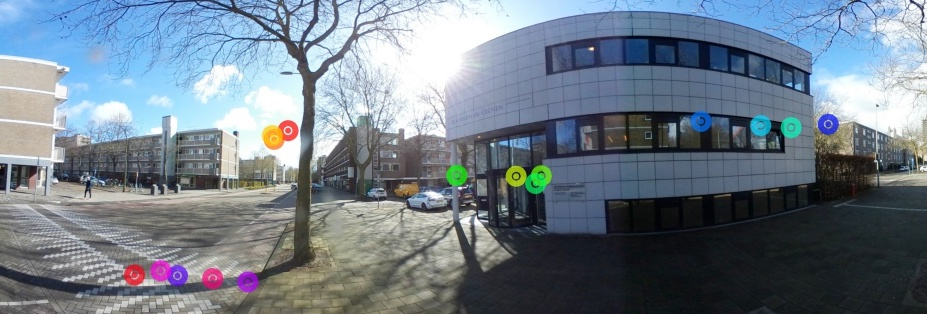
\includegraphics[width=\linewidth]{figures/2-met-video_sample.jpg}
        \caption{\DIFaddFL{Generated mock-up of the desired result of merged eye-tracking data of 16 participants, four groups with clear different behavior. See an animated example in the playlist at the start of this paper or }\href{https://youtube.com/playlist?list=PLzh4mA3kUCz2J9pJhzKEI88LiCYvB9BQk}{here}\DIFaddFL{.}}
        \label{fig:mapped-example}
    \end{figure}

    \DIFadd{As these methods are highly qualitative with an extensive workload for researchers, increasing the number of participants and gaining extra information directly increases the workload of extracting information, which could explain why the mentioned studies use between 5 }\DIFaddend and \DIFdelbegin \DIFdel{mapping several ofthese relative AOI's }\DIFdelend \DIFaddbegin \DIFadd{20 participants \mbox{%DIFAUXCMD
\cite{Rupi2019, Gruden2021, Trefzger2018}}\hspace{0pt}%DIFAUXCMD
. Gaining this information about differences might be helpful to provide insight into where multiple groups of participants are looking and possibly making distinctions between groups. It could be interesting, for example, to create a distinction between the viewing patterns or amount of tunnel vision of different age groups or using an e-bike or a regular city bicycle. While these kinds of distinctions can currently be made with wearable eye-trackers, their potential in decreasing researcher workload is considerable.
    }

    \DIFadd{As far as we could find, a combination of the different fields of wearable eye-tracking and panoramic imagery mapping does not yet exist. While existing software}\footnotemark \DIFadd{does enable multiple eye-trackers to be mapped to a similar point-based on image stills extracted from the frontal scene-cam, this is neither automated nor applicable for a longer duration, for example, tracking a full cycling itinerary or a traffic intersection with multiple participants. The mentioned existing eye-tracking studies contributed in the fields of, to name two, intersection design \mbox{%DIFAUXCMD
\cite{Rupi2019, Werneke2012, Kovacsova2018, Mantuano2017a} }\hspace{0pt}%DIFAUXCMD
and perception of danger in natural conditions \mbox{%DIFAUXCMD
\cite{Underwood2007, Liu2011, Lehtonen2016, VanGompel2007}}\hspace{0pt}%DIFAUXCMD
. These fields should be able extract more information quickly when the process of adding more participants and aggregating these data is streamlined. 
    }

    \footnotetext{\DIFadd{For example, the toolkit for the }\href{https://www.tobiipro.com/learn-and-support/learn/steps-in-an-eye-tracking-study/data/manual-and-assisted-mapping/}{TobiiPro} \DIFadd{wearable, which is proprietary software. }}

    \DIFadd{The absence of existing solutions leads us to the current project. In this research, a method is created to map a wearable eye-tracker }\DIFaddend on one single \DIFdelbegin \DIFdel{image is the topic where this project will focus on }\DIFdelend \DIFaddbegin \DIFadd{master image using a computer vision feature detection system. The relative gaze coordinates of wearable eye-trackers are mapped onto one single master footage. To determine where specific points are located on the "base image", we propose the usage of a one-shot image recognition architecture, in this case, a Siamese Neural Network (SNN), which we will introduce in }\autoref{sec:relatedworks}\DIFaddend . 

    \DIFaddbegin \DIFadd{To summarize, this paper aims to bring contribution to the following topics. 
    }

    \begin{itemize}
        \item \DIFadd{Expanding on the usefulness of eye-tracking in traffic interactions.
        }\item \DIFadd{Enabling a new research method by increasing the viable amount of participants in a wearable eye-tracking study.
        }\item \DIFadd{Evaluating the usefulness and accuracy of computer vision in mapping two images from streetscape together. 
    }\end{itemize}

    \subsection{\DIFadd{Research Questions}}
        \DIFadd{This research is divided into three research questions to establish concrete and measurable goals. RQ1 aims at establishing a baseline using a traditional computer vision algorithm. We will elaborate further on this method based on feature extraction, such as corner- and contrast-detection, in }\autoref{sec:traditionalcomputervision}\DIFadd{. We introduce this method to set a baseline for comparing the second method. For RQ2, we will introduce a SNN which takes a different approach, as explained in }\autoref{sec:snn}\DIFadd{. For RQ3, a video will be generated based on captured footage using the best functioning model. 
    }

        \begin{itemize}
            \item[RQ1] \DIFadd{How well can SIFT detect fragment location? 
            }\item[RQ2] \DIFadd{How well can a SNN detect fragment location?
            }\item[RQ3] \DIFadd{How can an aggregated AOI panoramic map of several wearable eye-trackers be created?
        }\end{itemize}

\DIFaddend \section{Related Works}\DIFaddbegin \label{sec:relatedworks}

    %DIF >  \subsection{Eye Tracking}
    %DIF >  Studies in \cite{St-Louis2014}

    \DIFaddend \subsection{\DIFdelbegin \DIFdel{Feature Detection \& Siamese Networks}\DIFdelend \DIFaddbegin \DIFadd{One-shot Image Recognition}\DIFaddend }
        Mapping several different images onto one master image without having the ability to train \DIFaddbegin \DIFadd{based on classical labeled examples (supervised learning) }\DIFaddend can be considered a case of one-shot image recognition. This problem is defined as being able to learn information about an object from one \DIFdelbegin \DIFdel{, }\DIFdelend or only a few \DIFdelbegin \DIFdel{, training samples /}\DIFdelend \DIFaddbegin \DIFadd{training samples or }\DIFaddend images \cite{WikipediaOneShotLearning2021}. It is a problem that humans are shown to be good at very quickly due to their ability to synthesize and learn new object classes from existing information about previously learned classes. This \DIFaddbegin \DIFadd{usage of previously learned knowledge }\DIFaddend is the key motivation for one-shot learning techniques, where systems can, as humans, use prior knowledge to classify new objects \cite{Fei-Fei2003, Fei-Fei2006}. \DIFdelbegin \DIFdel{This section will base partly on the explanation from \mbox{%DIFAUXCMD
\citeauthor{Koch2015} }\hspace{0pt}%DIFAUXCMD
in \mbox{%DIFAUXCMD
\cite{Koch2015}}\hspace{0pt}%DIFAUXCMD
.
        }%DIFDELCMD < 

%DIFDELCMD <         %%%
\subsection{\DIFdel{Traditional Computer Vision}}
        %DIFAUXCMD
\addtocounter{subsection}{-1}%DIFAUXCMD
\DIFdel{While this topic in computer vision has been addressed earlier in the 1980s and the 1990s, the basis }\DIFdelend \DIFaddbegin \DIFadd{The basis for this topic }\DIFaddend was laid by  \citeauthor{Fei-Fei2003} \cite{Fei-Fei2003}. In this paper, a variational Bayesian framework for one-shot image classification was created based on the idea that previously learned classes \DIFdelbegin \DIFdel{can }\DIFdelend \DIFaddbegin \DIFadd{could }\DIFaddend help forecast future ones. \DIFdelbegin \DIFdel{Traditional following computer }\DIFdelend \DIFaddbegin \DIFadd{Candidate architectures that are based on this principle might provide a solution direction. Computer }\DIFaddend vision models for one-shot learning \DIFdelbegin \DIFdel{usually fall into two categories: feature learning and }\DIFdelend \DIFaddbegin \DIFadd{are divided into either feature learning or }\DIFaddend metric learning. \DIFdelbegin \DIFdel{Example of both these types are respectively the Bag of Features (BoF) \mbox{%DIFAUXCMD
\cite{Wolf2009} }\hspace{0pt}%DIFAUXCMD
and }\DIFdelend \DIFaddbegin \DIFadd{In this project, we will build an implementation for both these categories. We will use the SIFT algorithm for the first, and the Siamese Neural Network for the second. 
        }

    \subsection{\DIFadd{Traditional Computer Vision}}
        \label{sec:traditionalcomputervision}
        \DIFaddend Scale-Invariant Feature Transform (SIFT) \DIFdelbegin \DIFdel{\mbox{%DIFAUXCMD
\cite{Lowe1999, Wan2013} }\hspace{0pt}%DIFAUXCMD
or Features from Accelerated Segment Test \mbox{%DIFAUXCMD
\cite{Rosten2006MachineDetection}}\hspace{0pt}%DIFAUXCMD
. }\DIFdelend \DIFaddbegin \DIFadd{works by first generating reference keypoints from a set of images, to which a new image is then compared  \mbox{%DIFAUXCMD
\cite{Low2004, Wan2013}}\hspace{0pt}%DIFAUXCMD
. The patent on this algorithm expired late 2020 and it is now incorporated in the OpenCV library \mbox{%DIFAUXCMD
\cite{OpenCV2020}}\hspace{0pt}%DIFAUXCMD
. By comparing the Euclidean distance (}{\color{blue}%DIFAUXCMD
\lstinline{cv.NORM_L2}%
}%DIFAUXCMD
\DIFadd{) between the detected keypoint vectors and comparing these to the new image, similarity between images can be identified. SIFT is selected because its generated keypoints are robust against several types of clutter, including different scaling, orientation, brightness, and partly to affine distortion. 
        }\DIFaddend 

        \DIFaddbegin \DIFadd{While SIFT can locate a fragment inside a global image, giving a definite position directly, we decided to evaluate both systems by the same method, opting to extract a similarity score instead. We believe this made the comparison between this method and the following method clearer. 
        }

    \DIFaddend \subsection{Siamese Neural Networks}
    \DIFaddbegin \label{sec:snn}
        \DIFaddend Another approach that uses the same core principle are Siamese Neural Networks (SNNs), which were first introduced by \citeauthor{Bromley1993} to solve the signature matching problem. \DIFaddbegin \DIFadd{This section is partly based on the explanation from \mbox{%DIFAUXCMD
\citeauthor{Koch2015} }\hspace{0pt}%DIFAUXCMD
in \mbox{%DIFAUXCMD
\cite{Koch2015}}\hspace{0pt}%DIFAUXCMD
. }\DIFaddend The core problem a SSN \DIFdelbegin \DIFdel{is aimed }\DIFdelend \DIFaddbegin \DIFadd{intends }\DIFaddend to solve is generating a robust representation in a multi-dimensional space, optimizing for a low distance between same-class objects \DIFdelbegin \DIFdel{, }\DIFdelend and a high distance between different objects. Training such a network is \DIFdelbegin \DIFdel{normally }\DIFdelend \DIFaddbegin \DIFadd{typically }\DIFaddend achieved by creating two \DIFdelbegin \DIFdel{augmentations of one image }\DIFdelend \DIFaddbegin \DIFadd{image augmentations}\DIFaddend , subject to certain conditions to avoid collapsing solutions \cite{Chen2020a}. 
        \DIFaddbegin 

        \begin{figure}
            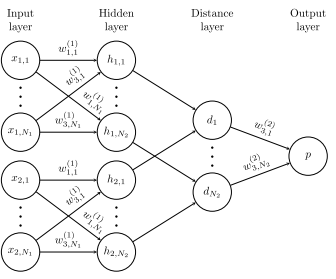
\includegraphics[width=\linewidth]{figures/1-rl-snn.png}
            \caption{\DIFaddFL{From \mbox{%DIFAUXCMD
\citeauthor{Koch2015} }\hspace{0pt}%DIFAUXCMD
\mbox{%DIFAUXCMD
\cite{Koch2015}}\hspace{0pt}%DIFAUXCMD
: Simple 2-hidden-layer Siamese Network for binary classification with logistic prediction $p$. Top and bottom networks are twins with shared weight matrices.}}
            \label{fig:1-rl-snn}
        \end{figure}

        \begin{figure}
            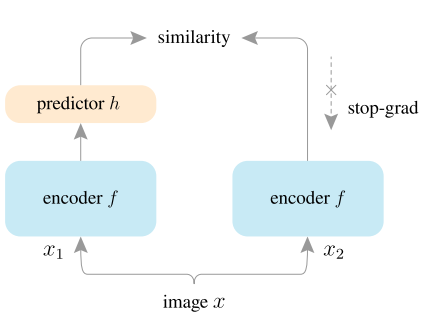
\includegraphics[width=\linewidth]{figures/1-rl-chen2020fig1.png}
            \caption{\DIFaddFL{SimSiam Architecture with a single predictor $h$ and stop-grad on the second twin, from \mbox{%DIFAUXCMD
\citeauthor{Chen2020a} }\hspace{0pt}%DIFAUXCMD
\mbox{%DIFAUXCMD
\cite{Chen2020a}}\hspace{0pt}%DIFAUXCMD
, page 1}}
            \label{fig:1-rl-chen2020fig1}
        \end{figure}

        \DIFaddend While many SNNs have been proposed and tried, a more typical SNN consists of two twin networks accepting different inputs, joined by an energy function at the top, see Figure~\DIFdelbegin \DIFdel{\ref{fig:simplesiamese}}\DIFdelend \DIFaddbegin \DIFadd{\ref{fig:1-rl-snn}}\DIFaddend . As visible, in this example, both networks use the same weight sets\DIFdelbegin \DIFdel{. This }\DIFdelend \DIFaddbegin \DIFadd{, which }\DIFaddend ensures both the consistency and symmetry of predictions, as both sides of the network will output the same function. 

        \DIFdelbegin %DIFDELCMD < \begin{figure}
%DIFDELCMD <             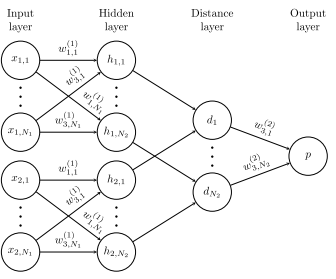
\includegraphics[width=\linewidth]{figures/siamesesimple.png}
%DIFDELCMD <             %%%
%DIFDELCMD < \caption{%
{%DIFAUXCMD
\DIFdelFL{From \mbox{%DIFAUXCMD
\citeauthor{Koch2015} }\hspace{0pt}%DIFAUXCMD
\mbox{%DIFAUXCMD
\cite{Koch2015}}\hspace{0pt}%DIFAUXCMD
: Simple 2-hidden-layer Siamese Network for binary classification with logistic prediction $p$. Top and bottom networks are twins with shared weight matrices.}}
            %DIFAUXCMD
%DIFDELCMD < \label{fig:simplesiamese}
%DIFDELCMD <         \end{figure}
%DIFDELCMD <         

%DIFDELCMD <         %%%
\DIFdel{While many versions exist, the }\DIFdelend \DIFaddbegin \DIFadd{The }\DIFaddend architecture used in this project was introduced by \citeauthor{Chen2020a}, called Simple Siamese Representation, short SimSiam. In \DIFdelbegin \DIFdel{this }\DIFdelend \DIFaddbegin \DIFadd{their }\DIFaddend paper, \citeauthor{Chen2020a} \DIFdelbegin \DIFdel{explores }\DIFdelend \DIFaddbegin \DIFadd{explore }\DIFaddend the effects of deliberately introducing a stop-gradient on the second "twin" of the SNN, which showed its effectiveness \cite{Chen2020a}. This version of a SNN showed an accuracy of 68.1\% \DIFaddbegin \DIFadd{on the ImageNet-dataset}\DIFaddend . The rest of this paragraph will briefly give an oversight of the structure of the used SNN as explained in \cite{Chen2020a} and \DIFdelbegin %DIFDELCMD < \autoref{fig:chen2020fig1}%%%
\DIFdelend \DIFaddbegin \autoref{fig:1-rl-chen2020fig1}\DIFaddend . The network takes in two random augmentations $x_1$ and $x_2$ from image $x$. The two images are processed by an encoder network $f$, which consists of a backbone (in this case, ResNet) and a projection Multilayer Perceptron (MLP). The encoder $f$ shares weights between the two views, as shown in \DIFdelbegin %DIFDELCMD < \autoref{fig:chen2020fig1}%%%
\DIFdelend \DIFaddbegin \autoref{fig:1-rl-chen2020fig1}\DIFaddend . Prediction head $h$ transforms the output of $f_1$ and matches it to the other unprocessed view $f_2$. In training, their cost function is defined as the negative cosine similarity between the two views. See for a detailed explanation \cite{Chen2020a}.   
        % Lots more explanation about neural networks and the specific type chosen in this paper to come here, using \cite{Roy2019} and \cite{Koch2015} as general sources and \cite{Chen2020}

\DIFdelbegin %DIFDELCMD < \begin{figure}
%DIFDELCMD <             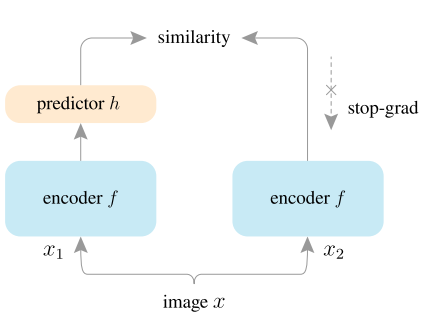
\includegraphics[width=\linewidth]{figures/chen2020fig1.png}
%DIFDELCMD <             %%%
%DIFDELCMD < \caption{%
{%DIFAUXCMD
\DIFdelFL{SimSiam Architecture, from \mbox{%DIFAUXCMD
\citeauthor{Chen2020a} }\hspace{0pt}%DIFAUXCMD
\mbox{%DIFAUXCMD
\cite{Chen2020a}}\hspace{0pt}%DIFAUXCMD
, page 1}}
            %DIFAUXCMD
%DIFDELCMD < \label{fig:chen2020fig1}
%DIFDELCMD <         \end{figure}
%DIFDELCMD <         

%DIFDELCMD <         
%DIFDELCMD < %%%
\section{\DIFdel{Research Question}}
    %DIFAUXCMD
\addtocounter{section}{-1}%DIFAUXCMD
\DIFdel{The question that is aimed to answer is as follows: 
}%DIFDELCMD < 

%DIFDELCMD <     \begin{quote}
%DIFDELCMD <         %%%
\DIFdel{How can an aggregated AOI 360-degree map of }%DIFDELCMD < \\ %%%
\DIFdel{several wearable eye trackers be created?
    }%DIFDELCMD < \end{quote}
%DIFDELCMD <     

%DIFDELCMD <     %%%
\subsection{\DIFdel{Sub questions}}
    %DIFAUXCMD
\addtocounter{subsection}{-1}%DIFAUXCMD
%DIFDELCMD < \begin{itemize}
\begin{itemize}%DIFAUXCMD
%DIFDELCMD <         \item %%%
\item%DIFAUXCMD
\DIFdel{How well does FAST (expand) detect fragment location? 
        }%DIFDELCMD < \item %%%
\item%DIFAUXCMD
\DIFdel{How well can a SNN detect fragment location?
    }
\end{itemize}%DIFAUXCMD
%DIFDELCMD < \end{itemize}
%DIFDELCMD <     

%DIFDELCMD < %%%
\DIFdelend \section{Methodology}\DIFdelbegin \DIFdel{To develop a proof of concept (PoC), the initial concept is taking one master-image in 360 degrees }\DIFdelend \DIFaddbegin \label{sec:methodology}
    \DIFadd{The initial concept of creating a heat-map takes one panoramic master image }\DIFaddend and using video footage from the wearable \DIFdelbegin \DIFdel{eye tracker }\DIFdelend \DIFaddbegin \DIFadd{eye-tracker }\DIFaddend to map on this image \DIFdelbegin \DIFdel{. A 360-degree }\DIFdelend \DIFaddbegin \DIFadd{as shown in }\href{https://www.youtube.com/playlist?list=PLzh4mA3kUCz2J9pJhzKEI88LiCYvB9BQk}{the example in this link}\DIFadd{. A panoramic }\DIFaddend image mainly exists in two forms: dual fish-eye, which is the raw output of two lenses on the camera, and equirectangular, which is a stitched and rectangular projection of the source. See an example of this behavior in \DIFdelbegin %DIFDELCMD < \autoref{fig:panoramicpic} %%%
\DIFdel{on page \pageref{fig:panoramicpic}}\DIFdelend \DIFaddbegin \autoref{fig:2-met-fisheye-stitched} \DIFadd{in the appendix on page \pageref{fig:2-met-fisheye-stitched}}\DIFaddend . To compare the \DIFdelbegin \DIFdel{eye tracker }\DIFdelend \DIFaddbegin \DIFadd{eye-tracker }\DIFaddend to this image, we will use the equirectangular projection. 

    \DIFdelbegin %DIFDELCMD < \begin{figure}
%DIFDELCMD <         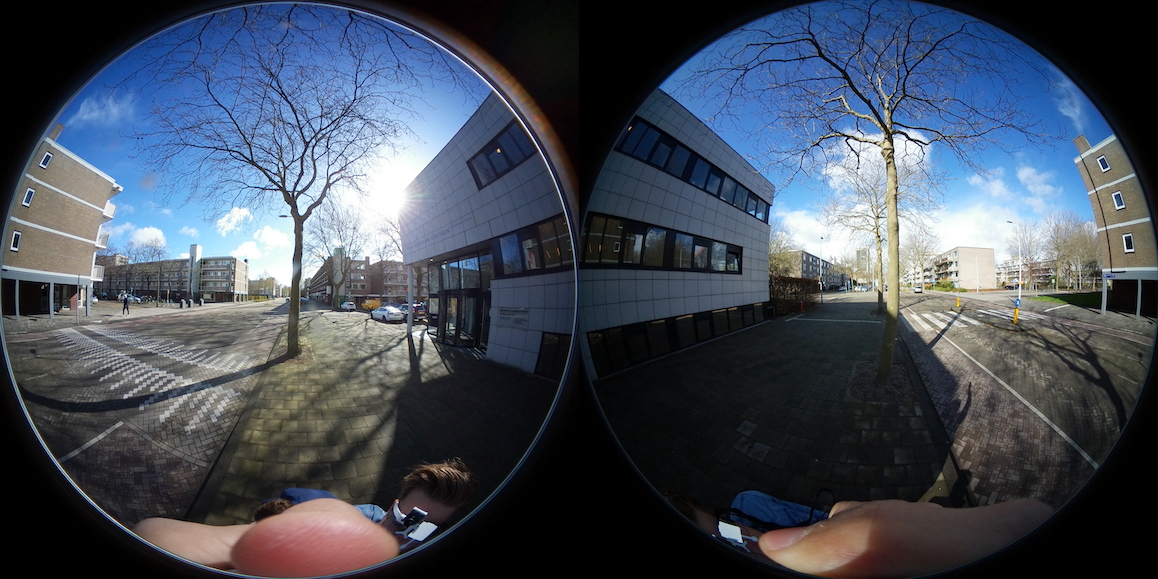
\includegraphics[width=\linewidth]{figures/1 original.JPG}
%DIFDELCMD <         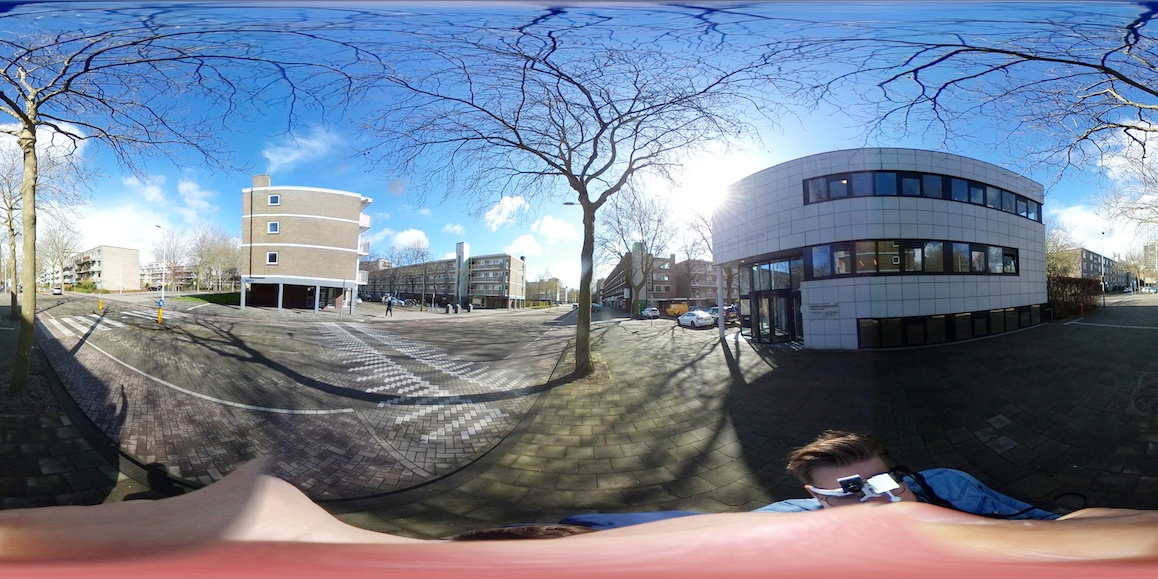
\includegraphics[width=\linewidth]{figures/2 stitchedunrolled.JPG}
%DIFDELCMD <         %%%
%DIFDELCMD < \caption{%
{%DIFAUXCMD
\DIFdelFL{Dual-fisheye (raw) and equirectangular footage}}
        %DIFAUXCMD
%DIFDELCMD < \label{fig:panoramicpic}
%DIFDELCMD <     \end{figure}
%DIFDELCMD <     

%DIFDELCMD <     %%%
\DIFdelend In this stage, the mapping will only work when the participant wearing the \DIFdelbegin \DIFdel{eye tracker }\DIFdelend \DIFaddbegin \DIFadd{eye-tracker }\DIFaddend is standing at the same point as the \DIFdelbegin \DIFdel{master-image was }\DIFdelend \DIFaddbegin \DIFadd{master image is }\DIFaddend created. As the \DIFdelbegin \DIFdel{eye tracker }\DIFdelend \DIFaddbegin \DIFadd{eye-tracker }\DIFaddend returns a JSON file with the estimated coordinates of the tracked pupil per frame, this can be mapped on the master image when its location is determined, see \DIFdelbegin %DIFDELCMD < \autoref{fig:simsiam-explan}%%%
\DIFdelend \DIFaddbegin \autoref{2-met-movinggrid}\DIFaddend . To compare and evaluate the different methods which will be tried, the footage from the \DIFdelbegin \DIFdel{eye tracker }\DIFdelend \DIFaddbegin \DIFadd{eye-tracker }\DIFaddend will have to be hand-labeled to establish ground truth. \DIFdelbegin \DIFdel{While traditional computer vision models can output an estimated location directly, a SNN needs to compare two images. In this case, every frame will be }\DIFdelend \DIFaddbegin \DIFadd{Every frame is }\DIFaddend compared to an extracted grid of \DIFdelbegin \DIFdel{unrolled }\DIFdelend footage of the \DIFdelbegin \DIFdel{360-degree }\DIFdelend \DIFaddbegin \DIFadd{panoramic }\DIFaddend camera, from which the most similar will be saved. The performance of \DIFdelbegin \DIFdel{the network }\DIFdelend \DIFaddbegin \DIFadd{both methods }\DIFaddend will be measured in \DIFaddbegin \DIFadd{the }\DIFaddend distance between the predicted position to the target (hand-labeled) position in pixels, where some margin can be taken in labeling a guess as \DIFdelbegin \DIFdel{a }\DIFdelend correct as the base frames will not always be a perfect fit.

    The workflow and procedure in this experiment \DIFdelbegin \DIFdel{is }\DIFdelend \DIFaddbegin \DIFadd{are }\DIFaddend therefore as follows: 

    \begin{enumerate}
        \item Grab \DIFaddbegin \DIFadd{panoramic }\DIFaddend image or video \DIFdelbegin \DIFdel{in 360-degree }\DIFdelend as master-track. 
        \item Unroll, stabilize\DIFdelbegin \DIFdel{and crop 360-degree }\DIFdelend \DIFaddbegin \DIFadd{, and crop panoramic }\DIFaddend footage.
        \item Collect \DIFdelbegin \DIFdel{eye tracker }\DIFdelend \DIFaddbegin \DIFadd{eye-tracker }\DIFaddend footage and data.
        \item Hand-label correct location of \DIFdelbegin \DIFdel{eye tracker }\DIFdelend \DIFaddbegin \DIFadd{eye-tracker }\DIFaddend footage.
        \item In case of SNN: Divide \DIFdelbegin \DIFdel{360-degree }\DIFdelend \DIFaddbegin \DIFadd{panoramic }\DIFaddend footage in excerpts to compare to \DIFdelbegin \DIFdel{eye tracker}\DIFdelend \DIFaddbegin \DIFadd{the eye-tracker footage}\DIFaddend .
        \item Compare the accuracy of different mapping methods.
    \end{enumerate}

    \subsection{Computer vision}
    Regarding the computer vision architectures, \DIFdelbegin \DIFdel{both SIFT and FAST were }\DIFdelend \DIFaddbegin \DIFadd{SIFT was }\DIFaddend selected as a baseline, using the existing open implementation by OpenCV2 \cite{OpenCV2020, OpenCV2020a}. For the SNN, an open-source implementation on Github with pre-trained weights was found and used\footnotemark.
    \footnotetext{See \url{https://github.com/taoyang1122/pytorch-SimSiam} for this implementation}

    \begin{figure}
        \DIFdelbeginFL %DIFDELCMD < \includegraphics[width=\linewidth]{figures/3 explanation.jpg}
%DIFDELCMD <         %%%
\DIFdelendFL \DIFaddbeginFL 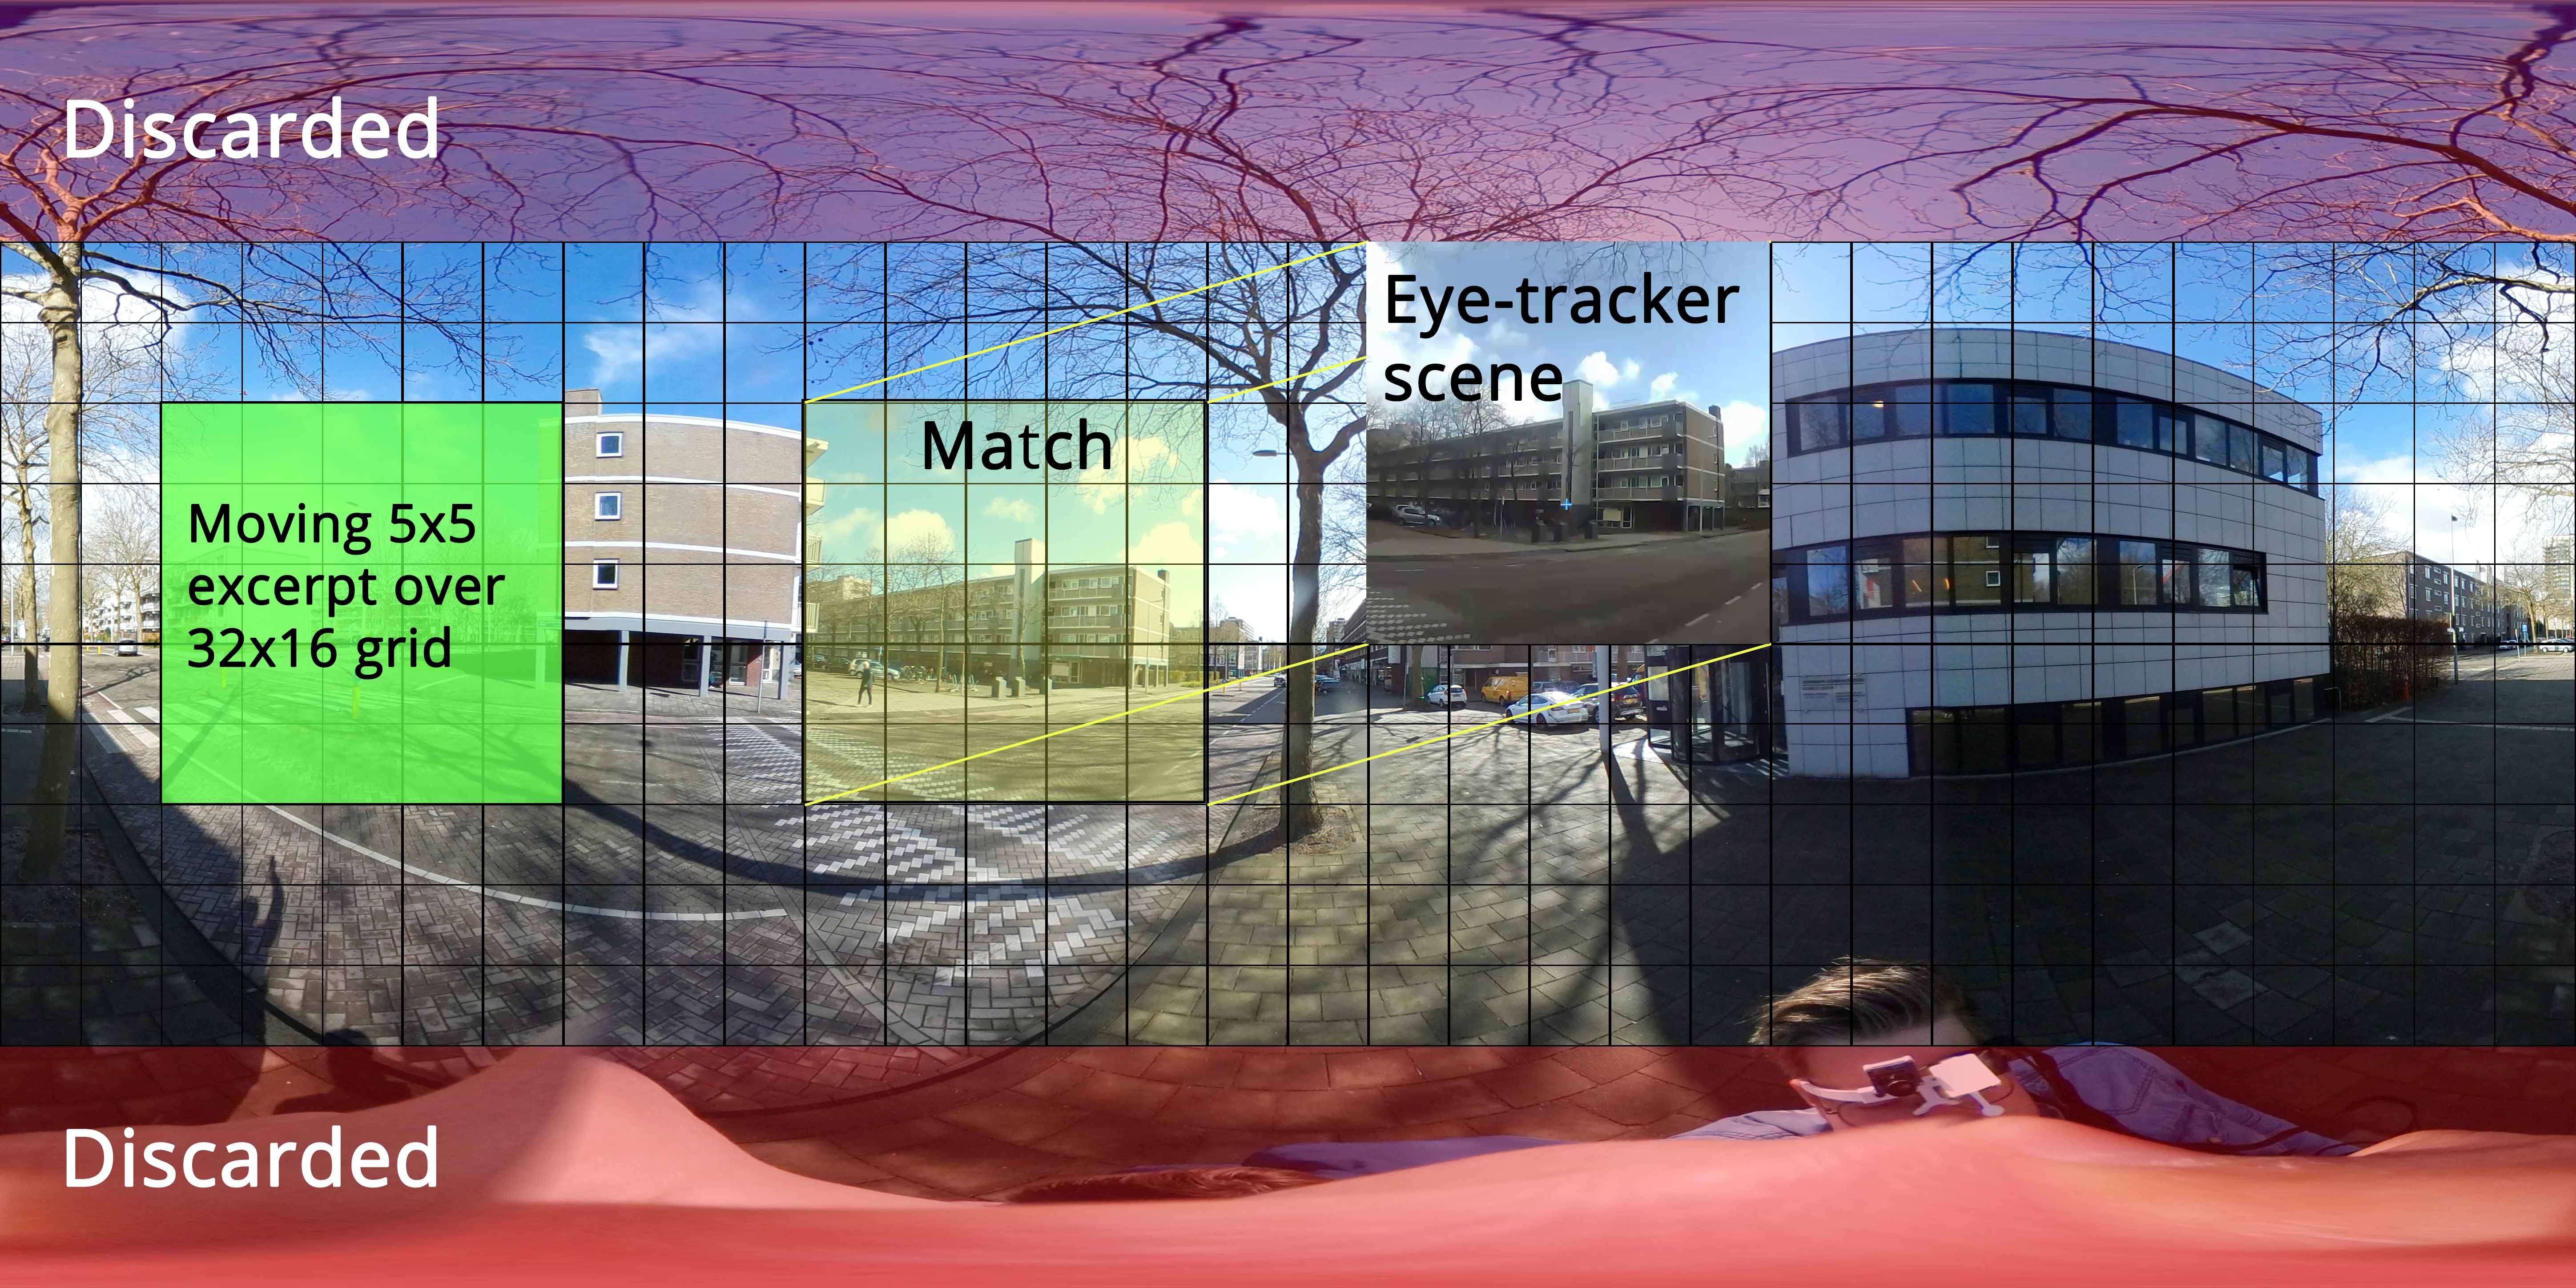
\includegraphics[width=\linewidth]{figures/2-met-movinggrid.jpg}
        \DIFaddendFL \caption{Visual explanation of comparison check.}
        \DIFdelbeginFL %DIFDELCMD < \label{fig:simsiam-explan}
%DIFDELCMD <     %%%
\DIFdelendFL \DIFaddbeginFL \label{2-met-movinggrid}
    \DIFaddendFL \end{figure}

\section{Experiments}
    \subsection{\DIFdelbegin \DIFdel{Kexxu OpenEye}\DIFdelend \DIFaddbegin \DIFadd{Hardware Used}\DIFaddend }
    The \DIFdelbegin \DIFdel{eye tracker }\DIFdelend \DIFaddbegin \DIFadd{eye-tracker }\DIFaddend used in this project is a beta-version of OpenEye, a prototype wearable \DIFdelbegin \DIFdel{eye tracker }\DIFdelend \DIFaddbegin \DIFadd{eye-tracker }\DIFaddend made by Kexxu, see \DIFdelbegin %DIFDELCMD < \autoref{fig:openeye}%%%
\DIFdelend \DIFaddbegin \autoref{3-exp-openeye} \DIFadd{on page \pageref{3-exp-openeye}}\DIFaddend . This version uses a pre-trained neural network on a \DIFdelbegin \DIFdel{wearable }\DIFdelend \DIFaddbegin \DIFadd{portable }\DIFaddend Raspberry PI to interpret pupil location in real-time\footnotemark. While it is normal for \DIFdelbegin \DIFdel{eye trackers }\DIFdelend \DIFaddbegin \DIFadd{eye-trackers }\DIFaddend to incorporate and distinguish between saccades and fixations \cite{VanGompel2007}, this \DIFdelbegin \DIFdel{eye tracker }\DIFdelend \DIFaddbegin \DIFadd{eye-tracker }\DIFaddend was not equipped with this capability. A 3D-printed wearable frame with one pupil-facing camera and one scene-facing camera are combined directly in one combined MP4 video file and a JSON file with relative focus positions. Every frame was center-cropped to 720x720 pixels to be used in the different image recognition methods. 
    \footnotetext{See \url{https://kexxu.com} for more details about the \DIFdelbegin \DIFdel{eye tracker }\DIFdelend \DIFaddbegin \DIFadd{eye-tracker }\DIFaddend used.} 

    \DIFaddbegin \begin{figure}
        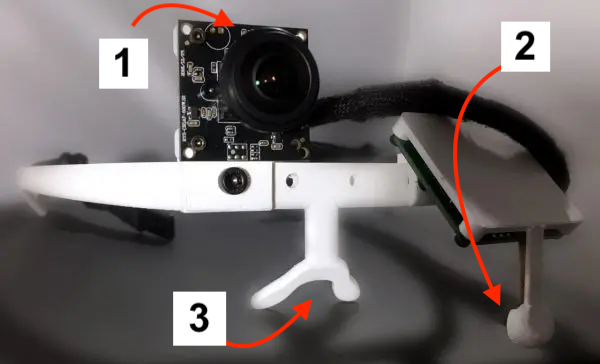
\includegraphics[width=\linewidth]{figures/3-exp-openeye.png}
        \caption{\DIFaddFL{OpenEye wearable consisting of (1) a scene-camera, (2) a left-eye facing camera and (3) the nose-bridge of the 3D-printed frame. }}
        \label{3-exp-openeye}
    \end{figure}

    \DIFaddend The footage grabbed for this Proof of Concept was 18 seconds of footage, a total of 245 frames, at a single location with an accurate embedded eye-tracking registration. The location for this initial test was in Amsterdam, near the office of Kexxu at the A. J. Ernststraat\DIFdelbegin \DIFdel{in Amsterdam}\DIFdelend . This is an urban location with plenty of possible features to be extracted. 

    \DIFdelbegin \subsection{\DIFdel{360-Degree Camera}}
        %DIFAUXCMD
\addtocounter{subsection}{-1}%DIFAUXCMD
\DIFdelend The camera used for grabbing the \DIFdelbegin \DIFdel{master-track}\DIFdelend \DIFaddbegin \DIFadd{master footage}\DIFaddend , in this case, a \DIFdelbegin \DIFdel{360-degree picture}\DIFdelend \DIFaddbegin \DIFadd{panoramic picture, }\DIFaddend is the Samsung Gear 360 II\DIFaddbegin \DIFadd{, }\DIFaddend which can grab both \DIFaddbegin \DIFadd{panoramic }\DIFaddend images and videos\DIFdelbegin \DIFdel{in 360-degrees}\DIFdelend \footnotemark. \footnotetext{For specifications, see \url{https://www.samsung.com/global/galaxy/gear-360/}.} 
        \DIFdelbegin \DIFdel{The footage generated by this camera was pre-processed using Cyberlink ActionDirector. 
        }\DIFdelend 

    \subsection{\DIFdelbegin \DIFdel{Image labeling}\DIFdelend \DIFaddbegin \DIFadd{Software Used}\DIFaddend }
    \DIFdelbegin \DIFdel{To label the correct position of each frame of the eye tracker camera, a simple }\DIFdelend \DIFaddbegin \DIFadd{A }\DIFaddend Flask-React service was built to hand-label the correct position \DIFdelbegin \DIFdel{and }\DIFdelend \DIFaddbegin \DIFadd{of each frame on the master footage and to }\DIFaddend validate the accuracy of several methods\footnotemark. \DIFaddbegin \DIFadd{The footage generated by the panoramic camera was pre-processed using Cyberlink ActionDirector, which offered the conversion to an equirectangular plane. Further processing and analysis is done in Jupyter Notebooks in a Conda-environment. 
    }\DIFaddend \footnotetext{See the GitHub repository for this service.}

\section{Results}
    \DIFdelbegin \subsection{\DIFdel{SIFT and FAST}}
        %DIFAUXCMD
\addtocounter{subsection}{-1}%DIFAUXCMD
\DIFdel{For trying out the functionality of SIFT and FAST, the recommended code by OpenCV was used . \mbox{%DIFAUXCMD
\cite{OpenCV2020, OpenCV2020a}}\hspace{0pt}%DIFAUXCMD
. A couple of samples were attempted, as seen in }\DIFdelend \DIFaddbegin \DIFadd{This section on results will give results ordered per research question and immediately discuss it. In the next section, Conclusions, we will summarize and close off. 
}

    \subsection{\DIFadd{RQ1: SIFT Performance}}
        \subsubsection{\DIFadd{Results}}
        \DIFadd{We used Scale-Invariant Feature Transform to establish a baseline to evaluate this classic computer vision architecture and compare the SNN effectively. Existing sample code fragments provided by the software package OpenCV were used to establish this section \mbox{%DIFAUXCMD
\cite{OpenCV2020, OpenCV2020a}}\hspace{0pt}%DIFAUXCMD
. In evaluating the accuracy, we used the same technique as in the Siamese Neural Network, in comparing fragment-wise (as shown in }\autoref{2-met-movinggrid}\DIFadd{) and selecting the image with the highest amount of matched keypoints as suggested by \mbox{%DIFAUXCMD
\cite{OpenCV2020}}\hspace{0pt}%DIFAUXCMD
. 
        }

        \DIFadd{All frames were compared using SIFT to the square extracts from the panoramic camera, where an accuracy within two frames from the target point of }\textbf{\DIFadd{52.03\%}} \DIFadd{was achieved. The locations where this algorithm fails to identify accurately seem to be darker images and images, including fewer overall keypoints. In }\DIFaddend \autoref{fig:sift-sample}\DIFdelbegin \DIFdel{on \pageref{fig:sift-sample}. 
        While these algorithms do get some points correct, these directions are not consistent enough to provide any real information. This method has not been attempted further than these samples. }\DIFdelend \DIFaddbegin \DIFadd{, the first image is correctly identified and the second and third incorrectly. For a comparison of more frames, see }\autoref{fig:4-res-comparisons} \DIFadd{on page~\ref{fig:4-res-comparisons}. 
        }\DIFaddend 

        \DIFaddbegin \begin{figure}
            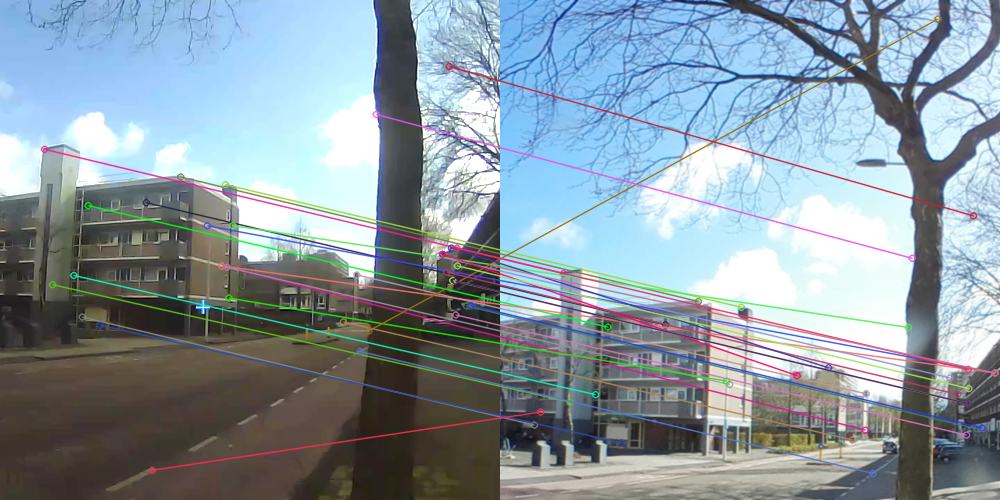
\includegraphics[width=\linewidth]{figures/4-sift1-048.png}
            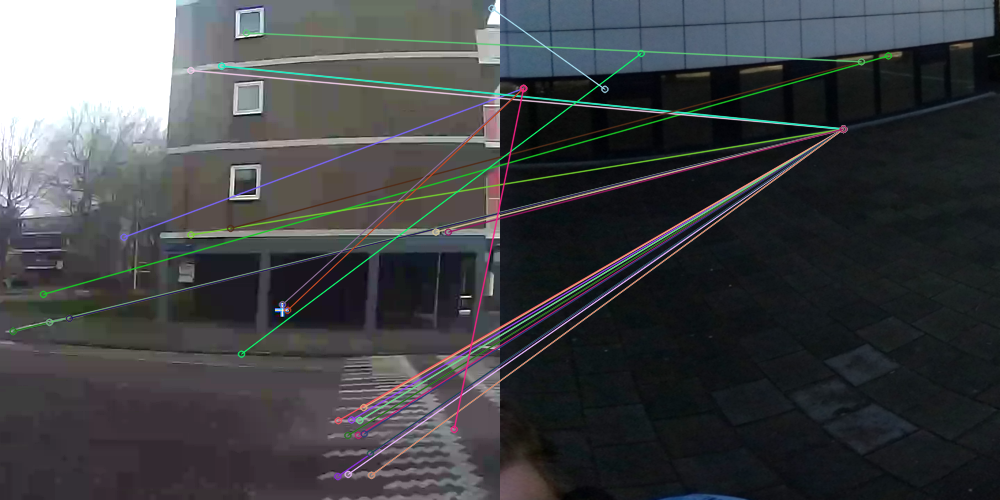
\includegraphics[width=\linewidth]{figures/4-sift2-117.png}
            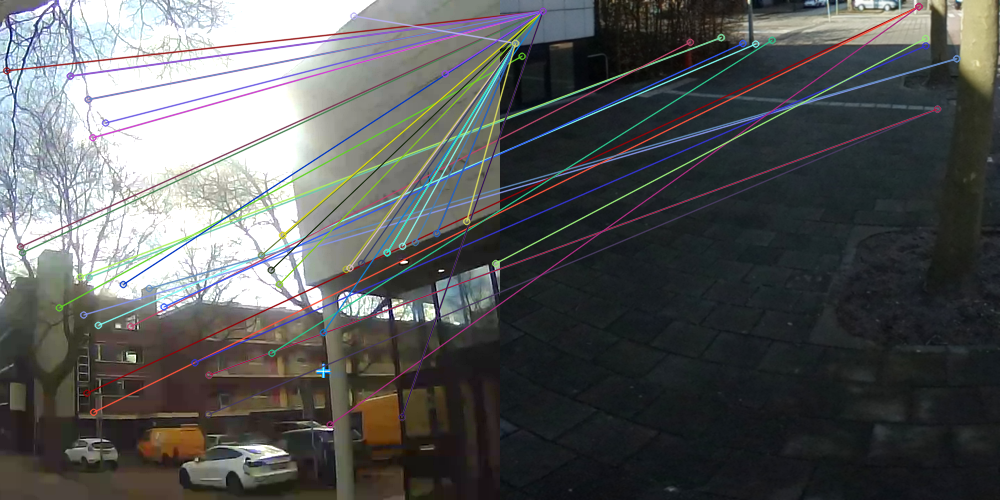
\includegraphics[width=\linewidth]{figures/4-sift3-143.png}
            \caption{\DIFaddFL{Three samples generated by SIFT: Left is the original eye-tracker scene camera, right is the estimated scene. }} 
            \label{fig:sift-sample}
        \end{figure} 

        \DIFaddend \subsubsection{Discussion}
        \DIFdelbegin \DIFdel{The lower scores generated by these methods can be explained by their designed nature. These size-invariant feature detection methods are great at detecting similar items based on corners, but the warped images generated by both the eye tracker and the 360-degree camera could have been a reason for this malfunction}\DIFdelend \DIFaddbegin \DIFadd{In the current setup, this method performed as expected, with some exceptions, such as the different affine transformations of the two different images and the difference in image quality. While SIFT is known to be resistant to scale and orientation, its ability to cope with different transformations as done by the transforming software of a panoramic camera is limited. This difference is evident when seeing the whole image, such as in }\autoref{2-met-movinggrid}\DIFadd{. One solution could be to, instead of mapping the panoramic footage on an equirectangular plane, mapping it on a projection based on the faces of a cube as done in \mbox{%DIFAUXCMD
\cite{Davidson2020}}\hspace{0pt}%DIFAUXCMD
. This alternative projection could reduce distortion and allow for better performance of this algorithm. 
        }

        \DIFadd{Another reason the algorithm fails to map some points correctly are the darker images in the master image. Darker spots in the images, such as the hard shadows generated by the low sun in the spring, can explain the tendency to be mapped to those points. An upside here is that these points of failure are usually sequentially between correctly mapped images, so smoothing could be applied to detect outlier image detection}\DIFaddend .  

    \subsection{\DIFaddbegin \DIFadd{RQ2: }\DIFaddend Siamese Network \DIFaddbegin \DIFadd{Performance}\DIFaddend }
        \DIFaddbegin \subsubsection{\DIFadd{Results}}
        \DIFaddend The SNN used has been pre-trained using the resources in the \DIFdelbegin \DIFdel{GitHub-repository. As explained in the methodology, all }\DIFdelend \DIFaddbegin \DIFadd{GitHub repository, which is the setup we will use here too. All }\DIFaddend 245 frames of the \DIFdelbegin \DIFdel{eye tracker were run through the SNN, as well as the grid of 31x5 }\DIFdelend \DIFaddbegin \DIFadd{eye-tracker and the grid of 32x6 }\DIFaddend extracts of the base image \DIFaddbegin \DIFadd{were run through the SNN}\DIFaddend . These images were compared using the negative cosine similarity metric as proposed in the original paper. \DIFaddbegin \DIFadd{The pre-training was done using batches of 432 with a learning rate of 0.1.
        }

        \DIFaddend Using this method, accuracy of estimation within 2 frames around the center track was created of \textbf{38.6\%}, see some examples and their scores (expressed as a \DIFaddbegin \DIFadd{fraction of a }\DIFaddend deviation of 181px, 1 frame) in \DIFdelbegin %DIFDELCMD < \autoref{fig:simsiam-sample} %%%
\DIFdel{on page \pageref{fig:simsiam-sample}. See a compiled estimated location of eye tracker frames on the master-track in the video on }%DIFDELCMD < \url{https://youtu.be/x9i05IzH_Cs}%%%
\DIFdel{. Distribution of the deviation from the target point in pixels is visible in }%DIFDELCMD < \autoref{fig:simsiam-deviation}%%%
\DIFdelend \DIFaddbegin \autoref{fig:4-res-comparisons} \DIFadd{on page \pageref{fig:4-res-comparisons}. }\DIFaddend . 

        \DIFdelbegin %DIFDELCMD < \begin{figure}
%DIFDELCMD <             \includegraphics[width=\linewidth]{figures/simsiam-deviation.png}
%DIFDELCMD <             %%%
%DIFDELCMD < \caption{%
{%DIFAUXCMD
\DIFdelFL{Binned amount of deviation from the target point. }}
            %DIFAUXCMD
%DIFDELCMD < \label{fig:simsiam-deviation}
%DIFDELCMD <         \end{figure}
%DIFDELCMD <     

%DIFDELCMD <         %%%
\DIFdelend \subsubsection{Discussion}
        \DIFdelbegin \DIFdel{While this SNN showed potential, its accuracy does seem too low. }\DIFdelend \DIFaddbegin \DIFadd{This early version of the SNN shows potential but performs worse than the baseline set by the SIFT algorithm. However, its potential is there, especially considering it is only trained based on object recognition from ImageNet. When implementing a version in follow-up research, focusing more on making streetscape comparisons could increase the accuracy, which can be trained using datasets such as \mbox{%DIFAUXCMD
\cite{Cordts2016TheUnderstanding}}\hspace{0pt}%DIFAUXCMD
. One other way of improving this neural network is by incorporating an algorithm correcting for the distorted lines in the equirectangular as done in \mbox{%DIFAUXCMD
\cite{Deng2017}}\hspace{0pt}%DIFAUXCMD
.
        }

        \DIFaddend As visible in \DIFdelbegin %DIFDELCMD < \autoref{fig:simsiam-deviation}%%%
\DIFdelend \DIFaddbegin \DIFadd{the graph in }\autoref{fig:4-res-deviation-distribution}\DIFaddend , a big part is within the \DIFdelbegin \DIFdel{2 }\DIFdelend \DIFaddbegin \DIFadd{two }\DIFaddend frames of deviation from the target position. This \DIFaddbegin \DIFadd{deviation }\DIFaddend is the part that \DIFdelbegin \DIFdel{could be explained , }\DIFdelend \DIFaddbegin \DIFadd{can be explained }\DIFaddend as similar features exist both in the source and target frame. The parts determined beyond the first spike are created by noise \DIFdelbegin \DIFdel{, and are incorrect}\DIFdelend \DIFaddbegin \DIFadd{and are inaccurate}\DIFaddend . These are, for example, the third, fourth\DIFdelbegin \DIFdel{and fifth image }\DIFdelend \DIFaddbegin \DIFadd{, and fifth images }\DIFaddend in the examples in \DIFdelbegin %DIFDELCMD < \autoref{fig:simsiam-sample}%%%
\DIFdelend \DIFaddbegin \autoref{fig:4-res-comparisons}\DIFaddend .

    \DIFdelbegin %DIFDELCMD < \begin{figure*}
%DIFDELCMD <         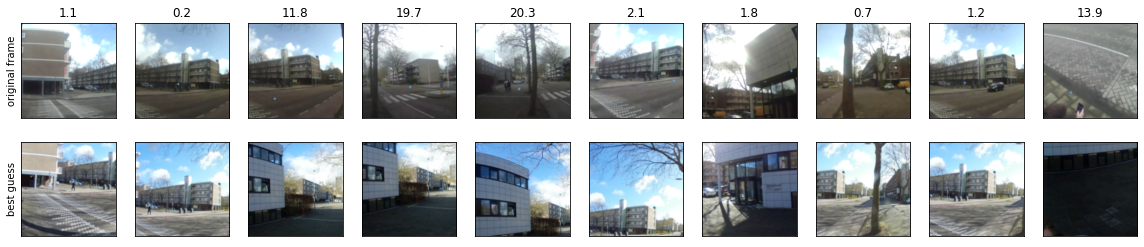
\includegraphics[width=\linewidth]{figures/simsiam-sample.png}
%DIFDELCMD <         %%%
\DIFdelendFL \DIFaddbeginFL \begin{figure}
        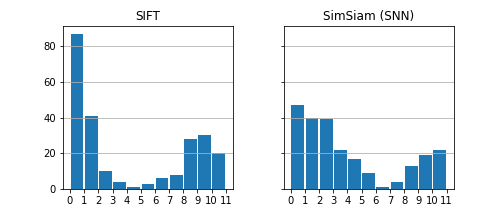
\includegraphics[width=\linewidth]{figures/4-res-deviation-distribution.png}
        \DIFaddendFL \caption{\DIFdelbeginFL \DIFdelFL{Frames and }\DIFdelendFL \DIFaddbeginFL \DIFaddFL{Distribution of }\DIFaddendFL distance \DIFdelbeginFL \DIFdelFL{(in frames) from }\DIFdelendFL \DIFaddbeginFL \DIFaddFL{of estimated fragments to }\DIFaddendFL the \DIFdelbeginFL \DIFdelFL{target }\DIFdelendFL \DIFaddbeginFL \DIFaddFL{true }\DIFaddendFL coordinates. \DIFaddbeginFL \DIFaddFL{Lower is better.}\DIFaddendFL }
        \DIFdelbeginFL %DIFDELCMD < \label{fig:simsiam-sample}
%DIFDELCMD <     \end{figure*}
%DIFDELCMD < %%%
\DIFdelend \DIFaddbegin \label{fig:4-res-deviation-distribution}
    \end{figure} 
    \DIFaddend 

    \DIFaddbegin \subsection{\DIFadd{RQ3: Creation of panoramic AoI-Map}}
        \subsubsection{\DIFadd{Results}}
        \DIFadd{The results of both methods are assembled into a video as proposed in }\autoref{sec:methodology}\DIFadd{, which is available on YouTube on the link below}\footnotemark\DIFadd{. See an example frame from one of the videos in }\autoref{fig:4-res-mapping-example}\DIFadd{. 
        }\footnotetext{\DIFadd{See  }\href{https://www.youtube.com/playlist?list=PLzh4mA3kUCz2J9pJhzKEI88LiCYvB9BQk}{youtube.com/playlist?list=PLzh4mA3kUCz2J9pJhzKEI88LiCYvB9BQk}\DIFadd{.}} 

        \begin{figure}
            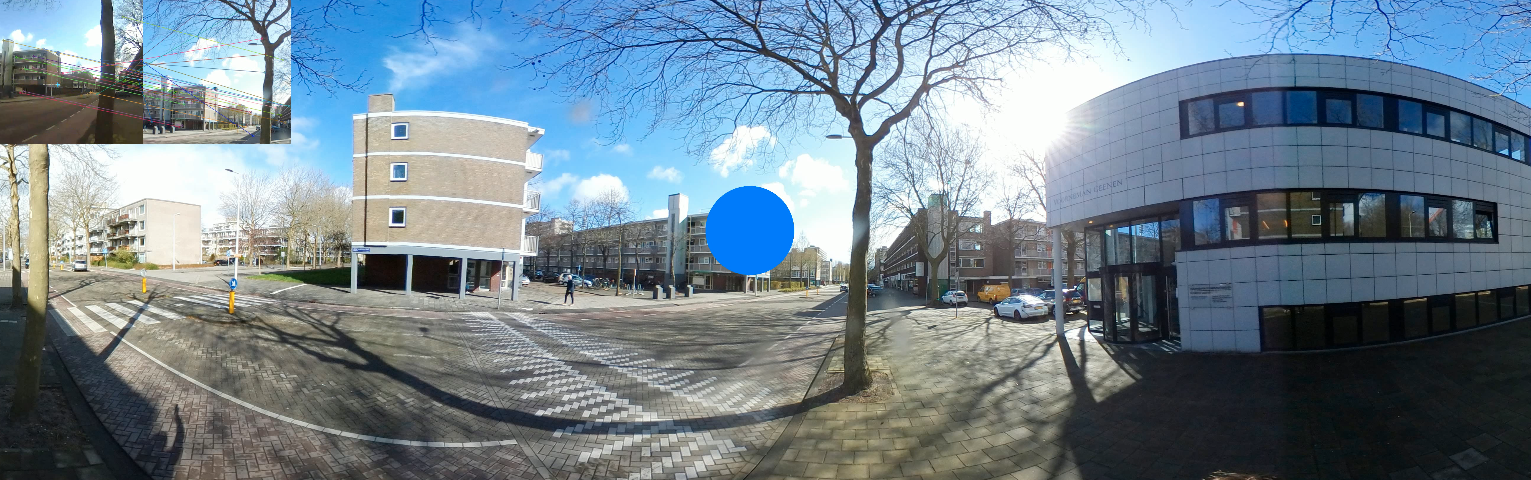
\includegraphics[width=\linewidth]{figures/4-res-mapping-example.png}
            \caption{\DIFaddFL{Example frame from the generated video, with a blue indicator positioned around the current gaze position.}}
            \label{fig:4-res-mapping-example}
        \end{figure} 

        \subsubsection{\DIFadd{Discussion}}
        \DIFadd{In both videos, the reliability of the used method is clearly visible, as the indicator of the current gaze position is not consistent. This could be done by interpolating the defined location. 
        }

        \DIFadd{When expanding this trial into the final goal of employing multiple eye-trackers on a shared itinerary, several other factors have to be considered. For one, both the master track and the individual itineraries should be recorded separately, with spatial location data available for each recorded frame. Using this, the correct master image that is closest can be determined. Another factor to consider is that all run itineraries should be run in relatively quick succession, as imagery and landscape can change, which can cause obstacles in the two different algorithms detecting the correct positions. 
}

\DIFaddend \section{Conclusion}
    \DIFdelbegin \DIFdel{While object }\DIFdelend \DIFaddbegin \DIFadd{Object }\DIFaddend detection by feature extraction \DIFdelbegin \DIFdel{is increasingly powerful, we have not been able to create a correctly functioning version }\DIFdelend \DIFaddbegin \DIFadd{seems more potent than the Siamese Neural Network, at least in this first version. This difference can be due to the SNN's nature, as only the standard pre-trained version was used }\DIFaddend in this project. \DIFdelbegin \DIFdel{While the SIFT and FAST networks showed potential, their output did not robustly show one position. The used }\DIFdelend \DIFaddbegin \DIFadd{The SIFT algorithm showed an accuracy of 52\% around the focus point. We hypothesize this accuracy should be enough to interpolate and make adjustments for the wrongly detected fragments using the sequential nature of the used video. While the used }\DIFaddend Siamese Neural Network \DIFdelbegin \DIFdel{has a showed }\DIFdelend \DIFaddbegin \DIFadd{shows an }\DIFaddend accuracy of 68.1\% \DIFaddbegin \DIFadd{in the original paper \mbox{%DIFAUXCMD
\cite{Chen2020a} }\hspace{0pt}%DIFAUXCMD
and thereby created big expectations}\DIFaddend , we reached an accuracy of 38.6\% within a margin of \DIFdelbegin \DIFdel{200 pixels around }\DIFdelend \DIFaddbegin \DIFadd{about 250 pixels centering }\DIFaddend the focus point. \DIFdelbegin \DIFdel{While it should be possible to make adjustments, such as integrating the dimension of time to improve these numbers, this was beyond the scope of }\DIFdelend \DIFaddbegin \DIFadd{We hope that a follow-up project can improve }\DIFaddend this \DIFaddbegin \DIFadd{accuracy and enable the research method as proposed in this }\DIFaddend project. 

\section{Acknowledgements}
    Thank you to Jurriaan Schreuder for providing resources and guidance for this thesis, and inspirational space to work with colleagues. I learned a lot while working on this project, for which I am thankful. A special thanks to the people I have discussed this idea with and who have provided me with guidance, such as Sander Buningh and Marco te Brommelstroet. Lastly, thank you to my supervisor at the University of Amsterdam: Marcel Worring for his \DIFaddbegin \DIFadd{quick and extensive }\DIFaddend feedback and supervision \DIFaddbegin \DIFadd{during this project}\DIFaddend . 

\DIFaddbegin \begin{landscape}
    \begin{figure}
        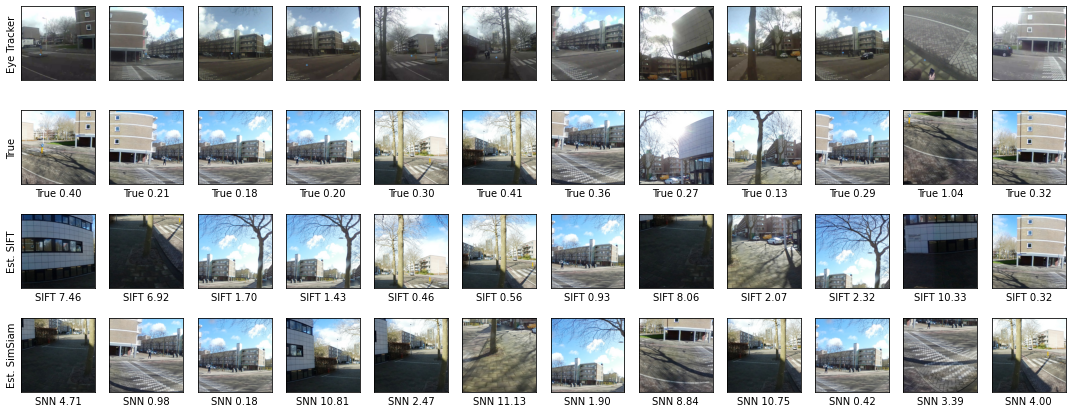
\includegraphics[width=\linewidth]{figures/4-res-comparisons.png}
        \caption{\DIFaddFL{Twelve sampled frames. Score (lower is better) is amount of }\emph{\DIFaddFL{excerpts}} \DIFaddFL{of deviation from the defined ground truth.}}
        \label{fig:4-res-comparisons}
    \end{figure} 
\end{landscape}

\DIFaddend % your refs
\section{References}
\printbibliography[heading=none]

\DIFdelbegin %DIFDELCMD < \begin{landscape}
%DIFDELCMD < %%%
\DIFdelend \appendix
\DIFdelbegin %DIFDELCMD < \begin{figure*}
%DIFDELCMD <         \includegraphics[width=\linewidth]{figures/SIFT1.png}
%DIFDELCMD <         \includegraphics[width=\linewidth]{figures/SIFT2.png}
%DIFDELCMD <         %%%
\DIFdelendFL \DIFaddbeginFL \section{\DIFaddFL{Panoramic projections}}
\begin{figure}[h]
    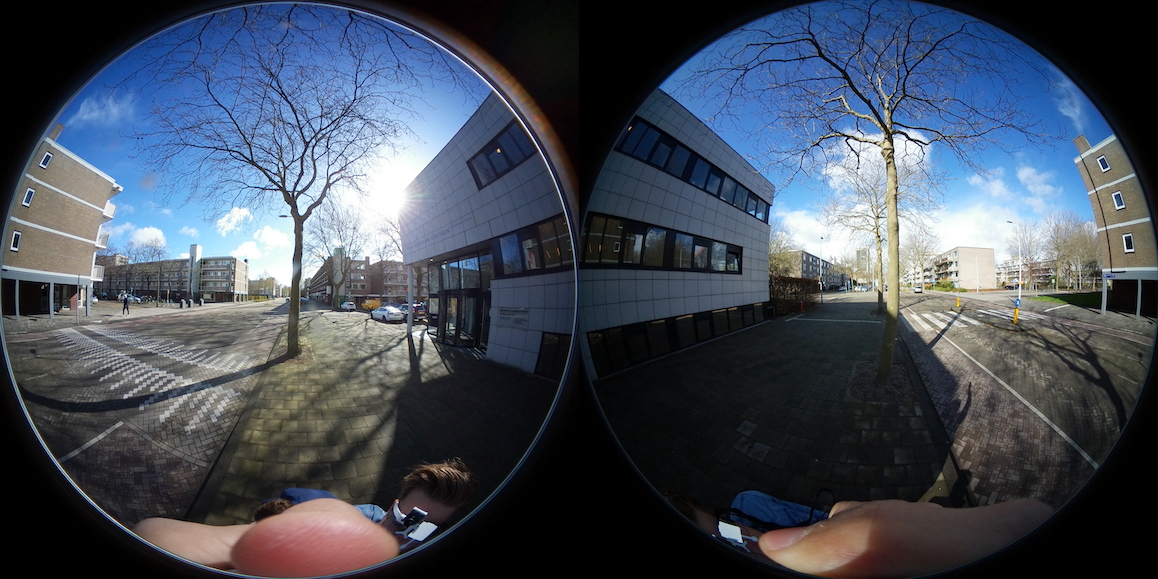
\includegraphics[width=\linewidth]{figures/2-met-fisheye.JPG}
    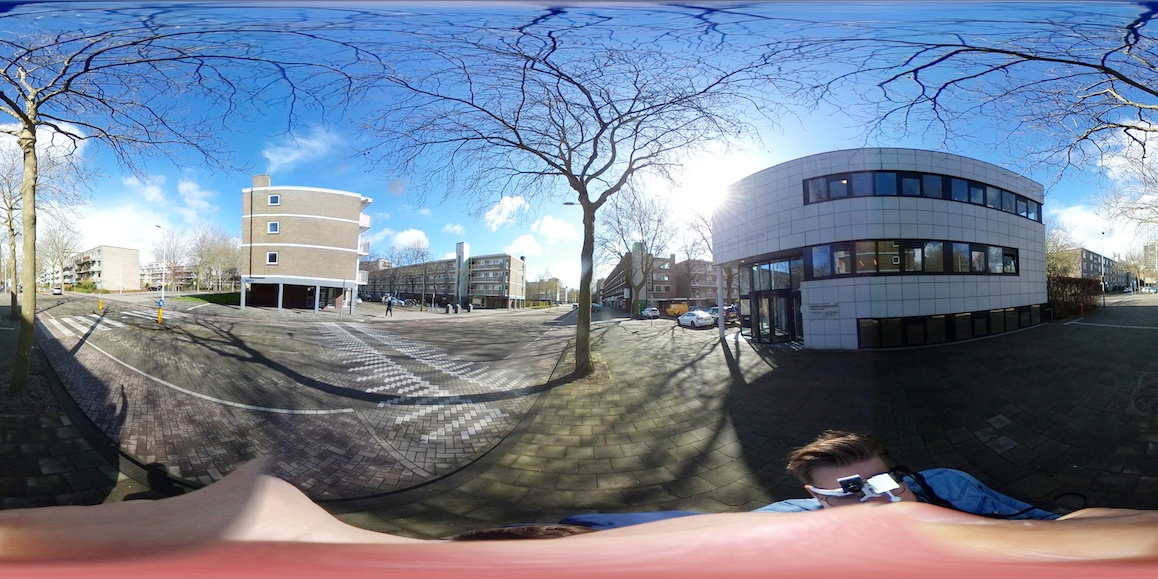
\includegraphics[width=\linewidth]{figures/2-met-stitched.JPG}
    \DIFaddendFL \caption{\DIFdelbeginFL \DIFdelFL{Two sample explorations using }\DIFdelendFL \DIFaddbeginFL \DIFaddFL{Behavior of a fish-eye capture and }\DIFaddendFL the \DIFdelbeginFL \DIFdelFL{SIFT feature extraction}\DIFdelendFL \DIFaddbeginFL \DIFaddFL{equirectangular flat render}\DIFaddendFL .}
    \DIFdelbeginFL %DIFDELCMD < \label{fig:sift-sample}
%DIFDELCMD <     \end{figure*}
%DIFDELCMD < \end{landscape}
%DIFDELCMD < %%%
\DIFdelend \DIFaddbegin \label{fig:2-met-fisheye-stitched}
\end{figure}
\DIFaddend 

\end{document}